% \section{Long-term (1985 – 2018) monitoring of forest cover changes in the Atlantic Forest using Landtrendr algorithm}
\section{Monitoramento de longo prazo (1985 – 2018) das mudanças florestais na Mata Atlântica utilizando o algoritmo Landtrendr}
\subsection{Introdução}
\hspace{13pt} Introdução.

\subsection{Materiais e Métodos}
\subsubsection{Área de estudo}
\hspace{13pt} O estudo abrange toda a área do bioma da Mata Atlântica brasileira (Figura \ref{fig:mata_atlantica}), que possui atualmente uma área total de aproximadamente 1.1 Mkm2 ou 110 Mha. O bioma está presente em 15 estados brasileiros e é onde se localiza grande parte da atividade econômica e população do pais. Atualmente, vivem na Mata Atlântica cerca de 72\% da população brasileira, o que em parte explica o fato de hoje apenas cerca de 12\% de sua cobertura natural ter persistido.. O bioma ainda possui 75,6\% das espécies ameaçadas e endêmicas do Brasil, o que o torna um dos mais prioritários para conservação no país. Além disso, estima-se que entre 43\% e 45\% do total de espécies de plantas e vertebrados sejam restritas a esse bioma \citep{scarano2014}.

\begin{figure}[h!]
    \centering
    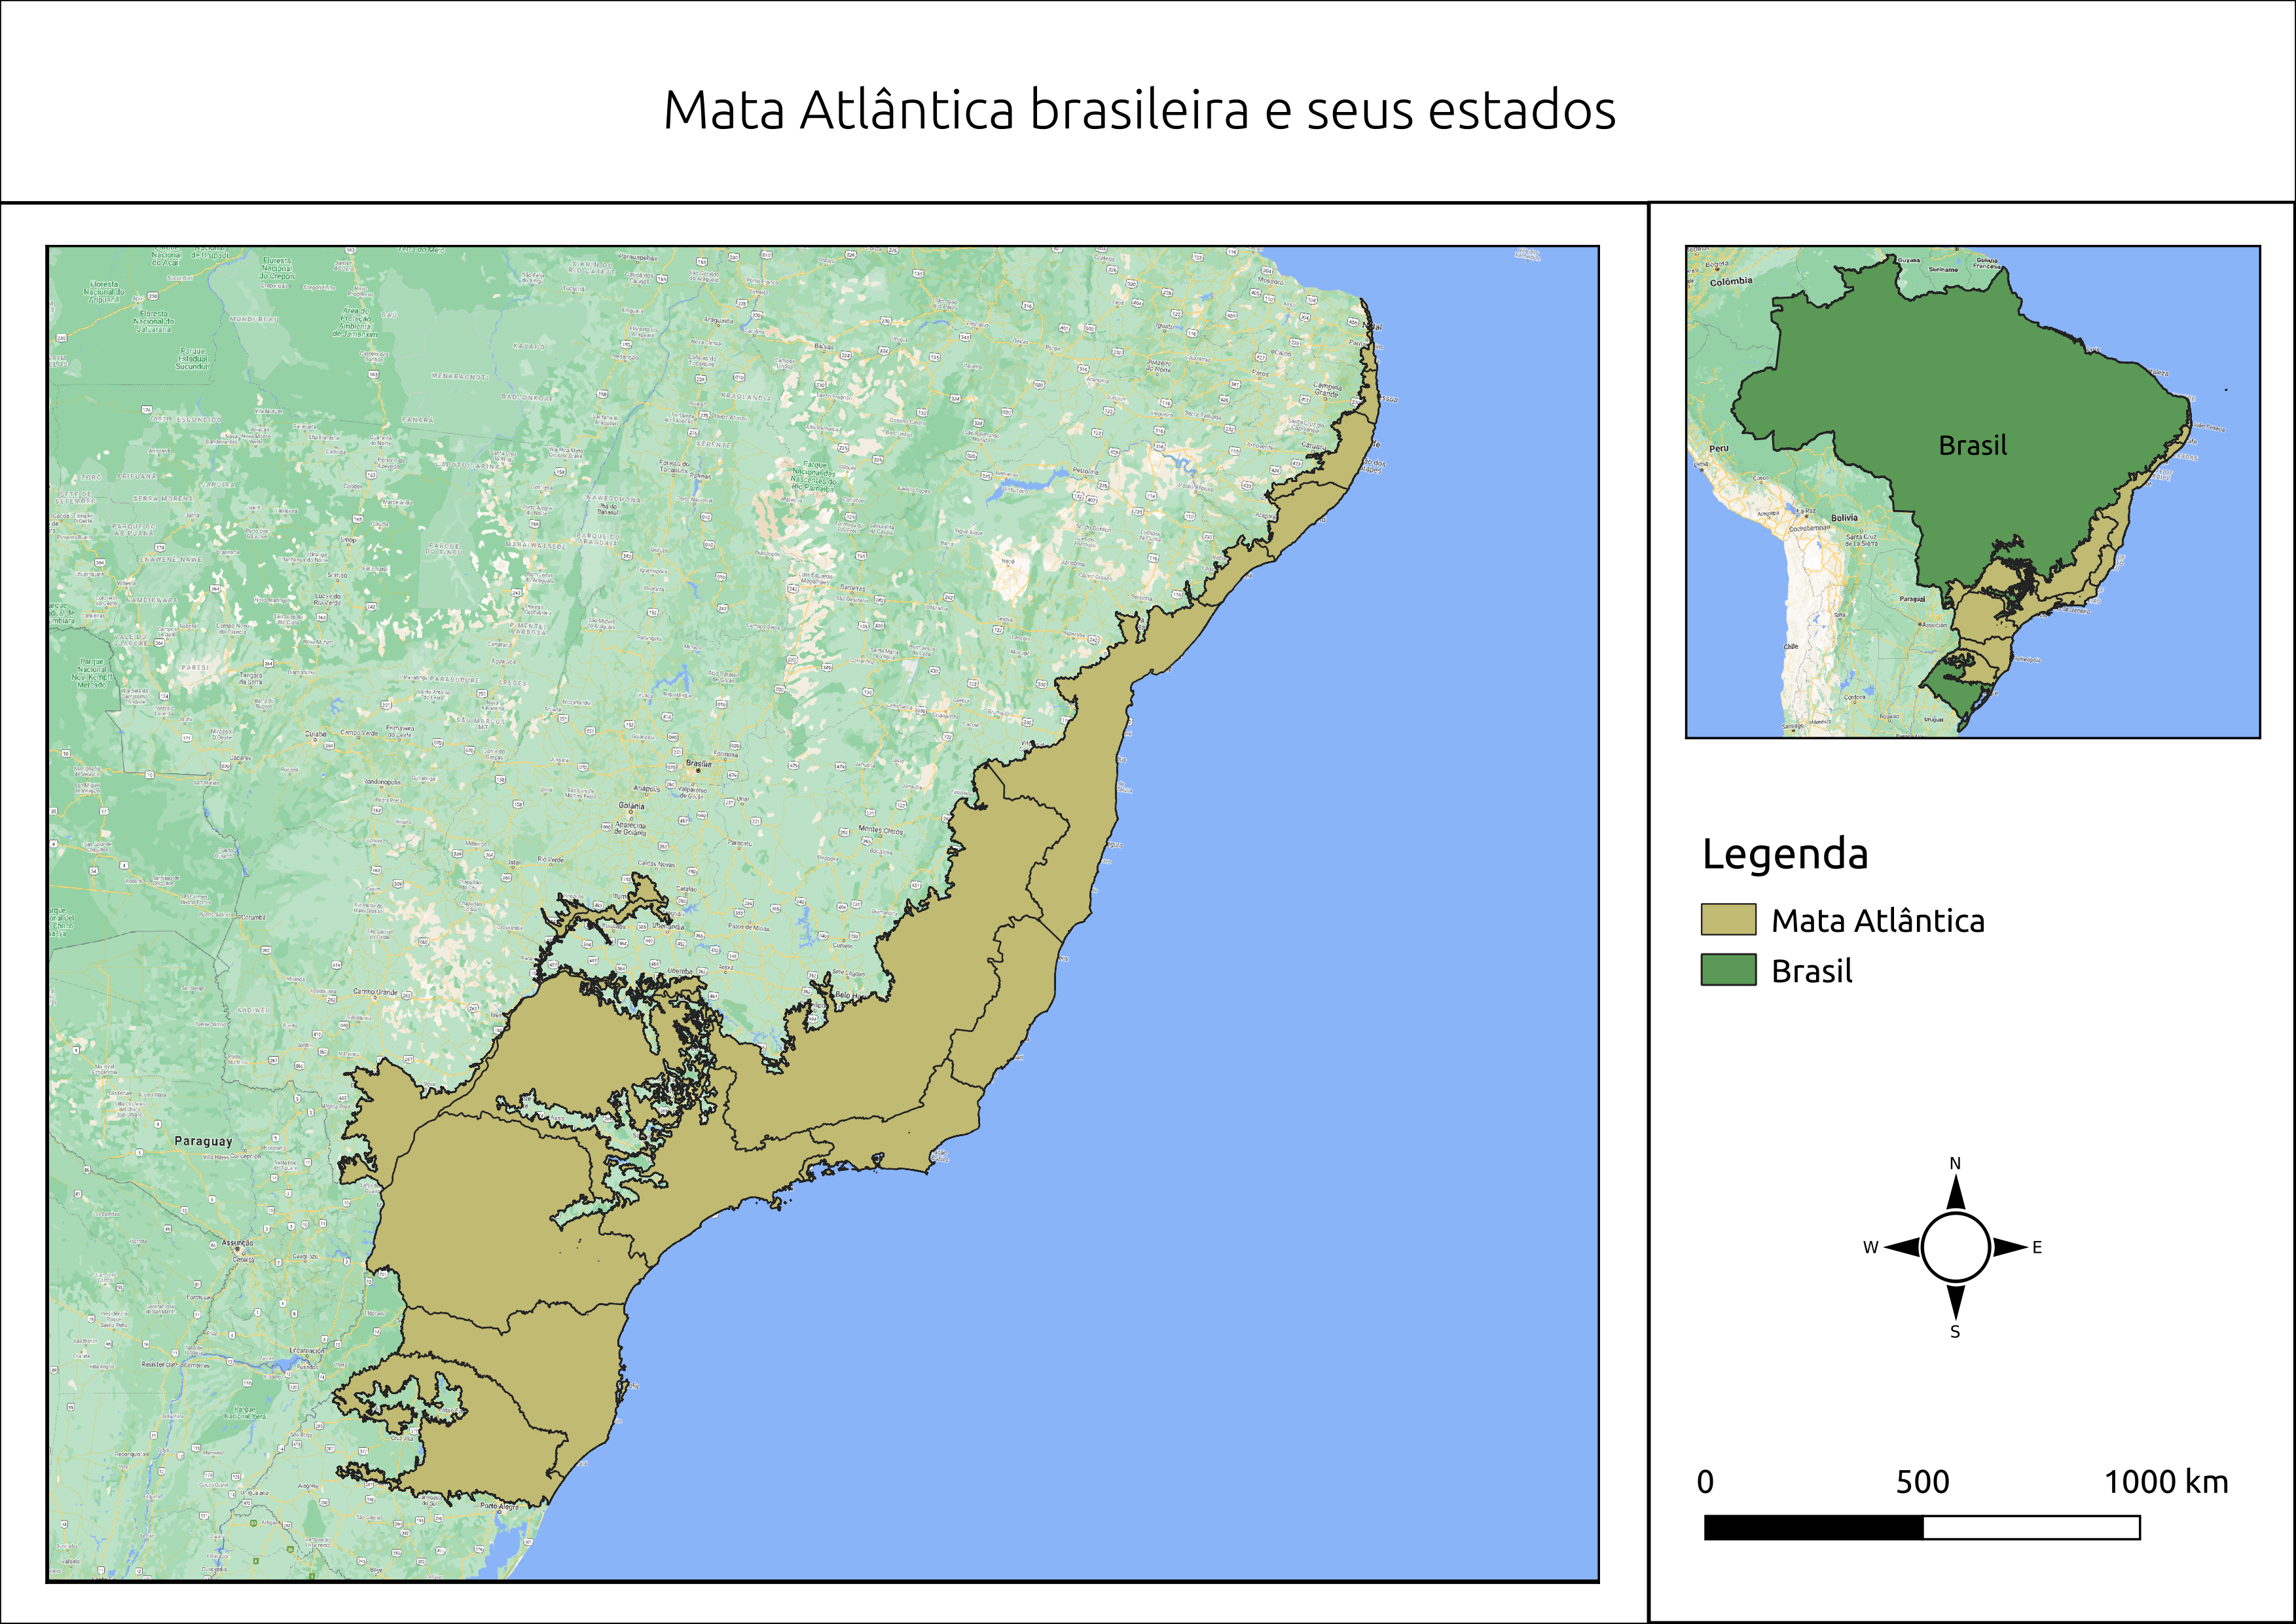
\includegraphics[scale=.5]{images/mata_atlantica.png}
    \caption{Área de Estudo - Mata Atlântica brasileira}
    \label{fig:mata_atlantica}
\end{figure}

Na época da chegada dos portugueses no Brasil, a Mata Atlântica cobria cerca de 1,5 milhões de quilômetros quadrados, estendendo-se ao longo de 3 mil quilômetros da costa brasileira - do Rio Grande do Sul ao Rio Grande do Norte - e penetrando pelo interior, cruzando São Paulo, Minas Gerais e Mato Grosso do Sul até as fronteiras da Argentina e do Paraguai \citep{scarano2014}. Cerca de 500 anos depois, esse extenso e representativo bioma abriga mais de 100 milhões de pessoas, cerca de 1/4 das quais ainda vivem na pobreza \citep{scarano2014}.

Segundo o projeto Mapbiomas, a área total de florestas no bioma em 1985 era de X e em 2018 de X. Já a área de florestas que não sofreram mudanças significativas (pseudo-invariantes) durante o período de 1985 até 2018 foi de aproximadamente 21.4 Mha. Deste total, somente  30\% da vegetação nativa remanescente está protegida legalmente através de unidades de conservação.

% Apesar dos importantes avanços obtidos nesta agenda na última década – como a restauração de aproximadamente 1,4 milhões de hectares entre 2011 e 2020 – muito ainda precisa ser feito \citep{CROUZEILLES2019}

\subsubsection{Dados de entrada}
\hspace{13pt} Para o mapeamento do bioma consideramos um intervalo anual que compreendeu todos os anos de 1985 até 2018 utilizando imagens do satélite Landsat das séries 5, 7 e 8. A escolha desse período de análise se deu por conta do início da captura de dados iniciado em 1 de março de 1984 pelo satélite Landsat 5 e consequente disponibilidade de dados pela comunidade científica para o mesmo período, o que facilitou a verificação e validação dos resultados. Para cobrir todos os 110 Mha do bioma foi necessário a compilação e processamento de 88 cenas Landsat, cada uma com cerca de 23 imagens com por ano, o que dá algo em torno de 67 mil imagens. Se considerarmos que cada uma dessas imagens possui pelo menos 7 bandas, chegamos a um cubo multidimensional de quase meio milhão de bandas. Um processamento que sem dúvidas só seria possível com o advento das tecnologias já citadas.

Todas as imagens utilizadas são da coleção \emph{surface reflectance}, o que significa que já possuem correção geométrica, radiométrica e possuem valor físico referente a superfície terrestre. Além disso, as imagens passaram por processo de harmonização para evitar acúmulo de ruídos. As séries temporais foram criadas utilizando uma função própria do Landtrendr.

\subsubsection{Método de análise}
\hspace{13pt} A análise das trajetórias foi feita utilizando o algoritmo Landtrendr em sua versão para a plataforma Google Earth Engine (GEE) \citep{Kennedy2018}. As vantagens da implementação do algoritmo no GEE em relação a sua versão original em ENVI/IDL está na possibilidade de sua aplicação em áreas extensas. Além disso, a versão para GEE elimina grande parte dos desafios técnicos presentes em sua implementação clássica. No entanto, apesar do ganho significativo no tempo de processamento quando comparado a sua versão em IDL, o Landtrendr GEE também apresenta algumas limitações. Uma das maiores está na limitação na extensão da análise para apenas uma imagem Landsat por vez. A plataforma apresentou erros sistemáticos quando foi requisitada para processar análises para toda a Mata Atlântica de uma só vez, por exemplo. Com isso, o processamento teve de ser feito em etapas. 

Com isso, as etapas tiveram de ser divididas por cenas Landsat, neste caso, 88 cenas (Figura \ref{fig:pathrow_centroids}). Como o resultado do algoritmo é dado de forma separada por cena, foi necessário juntar todas as camadas geradas em uma única após uma etapa extra de pós-processamento. Devido a ruídos presentes nas bordas das imagens Landsat e a sobreposição natural entre imagens diferentes, nem todos os pixels presentes nas bordas apresentaram resultados similares. Juntar todos as 88 camadas de resultados em uma se tornou um desafio e só foi possível através criação de polígonos de voronoi \citep{Okabe}, o que possibilitou utilizarmos somente as áreas mais próximas do centro das camadas geradas pelo algoritmo. 

\begin{figure}[h!]
    \centering
    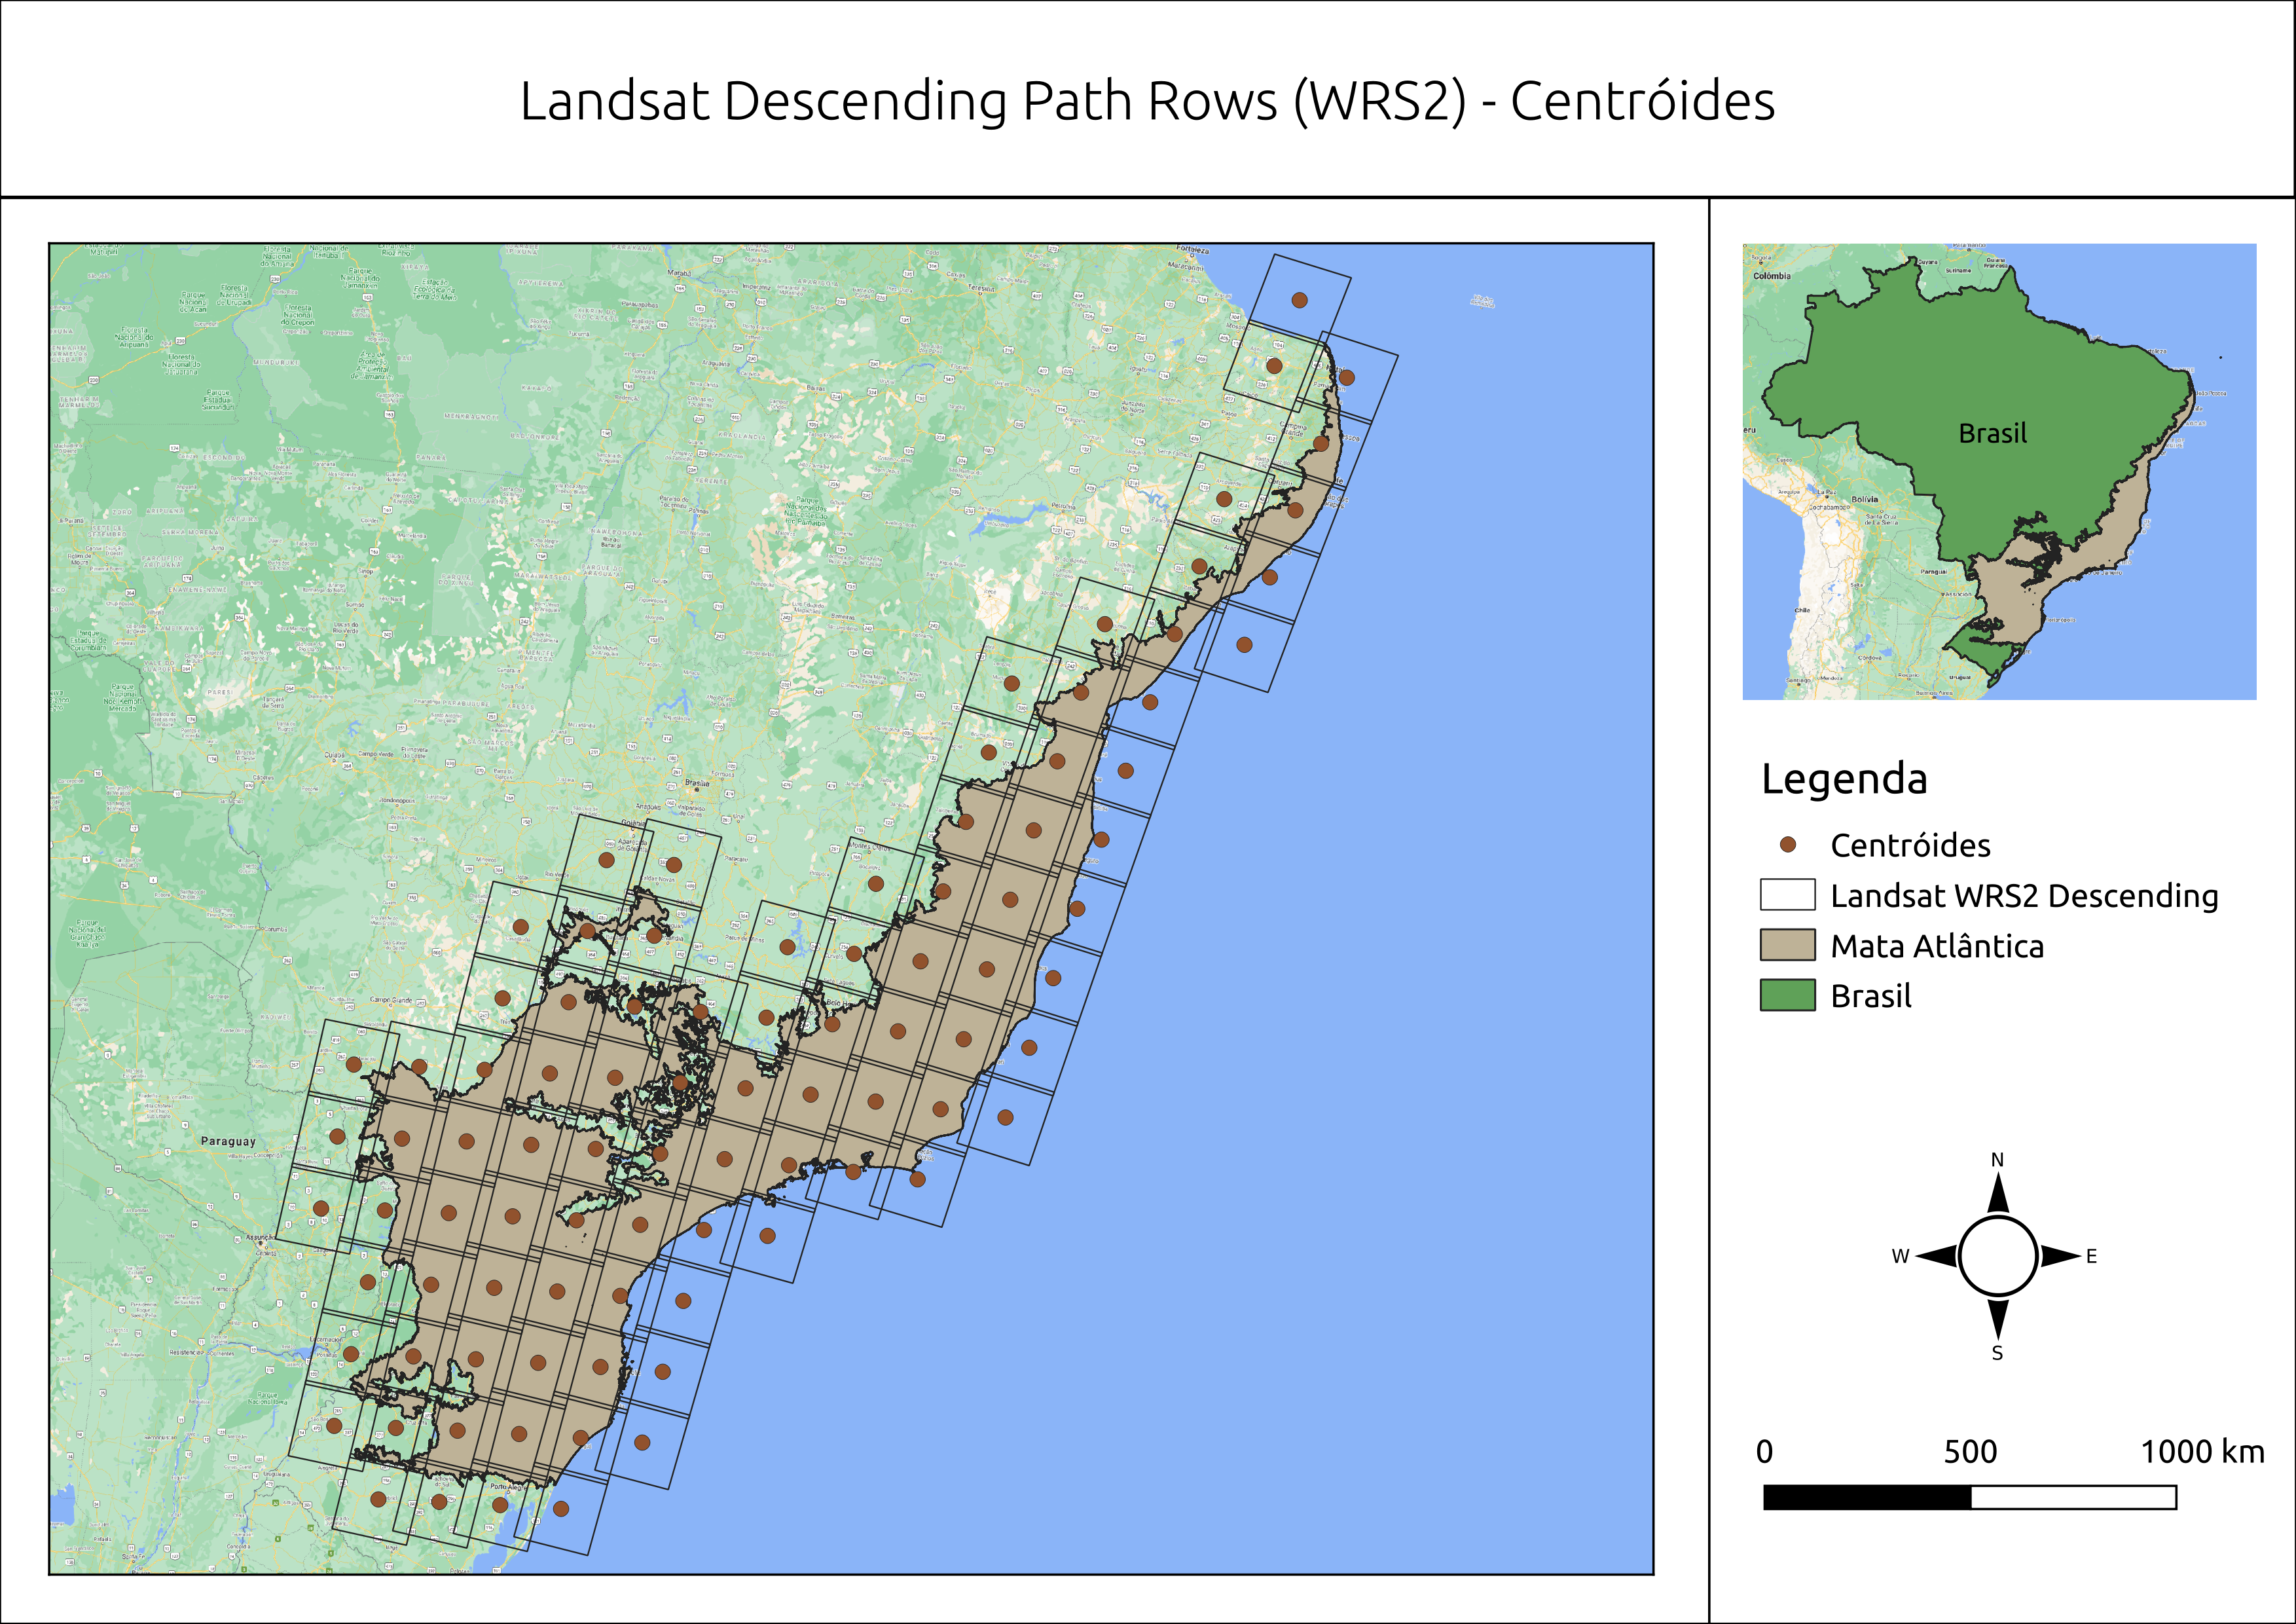
\includegraphics[scale=.5]{images/ma_pathrow_centroids.png}
    \caption{Pathrows das imagens Landasat e seus respectivos centróides que foram utilizados para delimitar as cenas a serem processadas pelo algoritmo}
    \label{fig:pathrow_centroids}
\end{figure}

Os polígonos de voronoi foram gerados através da extração dos centroides dos polígonos delimitadores das cenas Landsat e posteriormente utilizados para a criação dos polígonos com as áreas centrais (Figura \ref{fig:voronoi_ma}). Após a geração dos polígonos de voronoi, os mesmos foram utilizados para recordar os resultados de forma a limpar possíveis sobreposições. Após o recorte, todas as imagens foram agregadas para toda extensão do bioma e separadas banda a banda para análise posterior.

\begin{figure}[H]
    \centering
    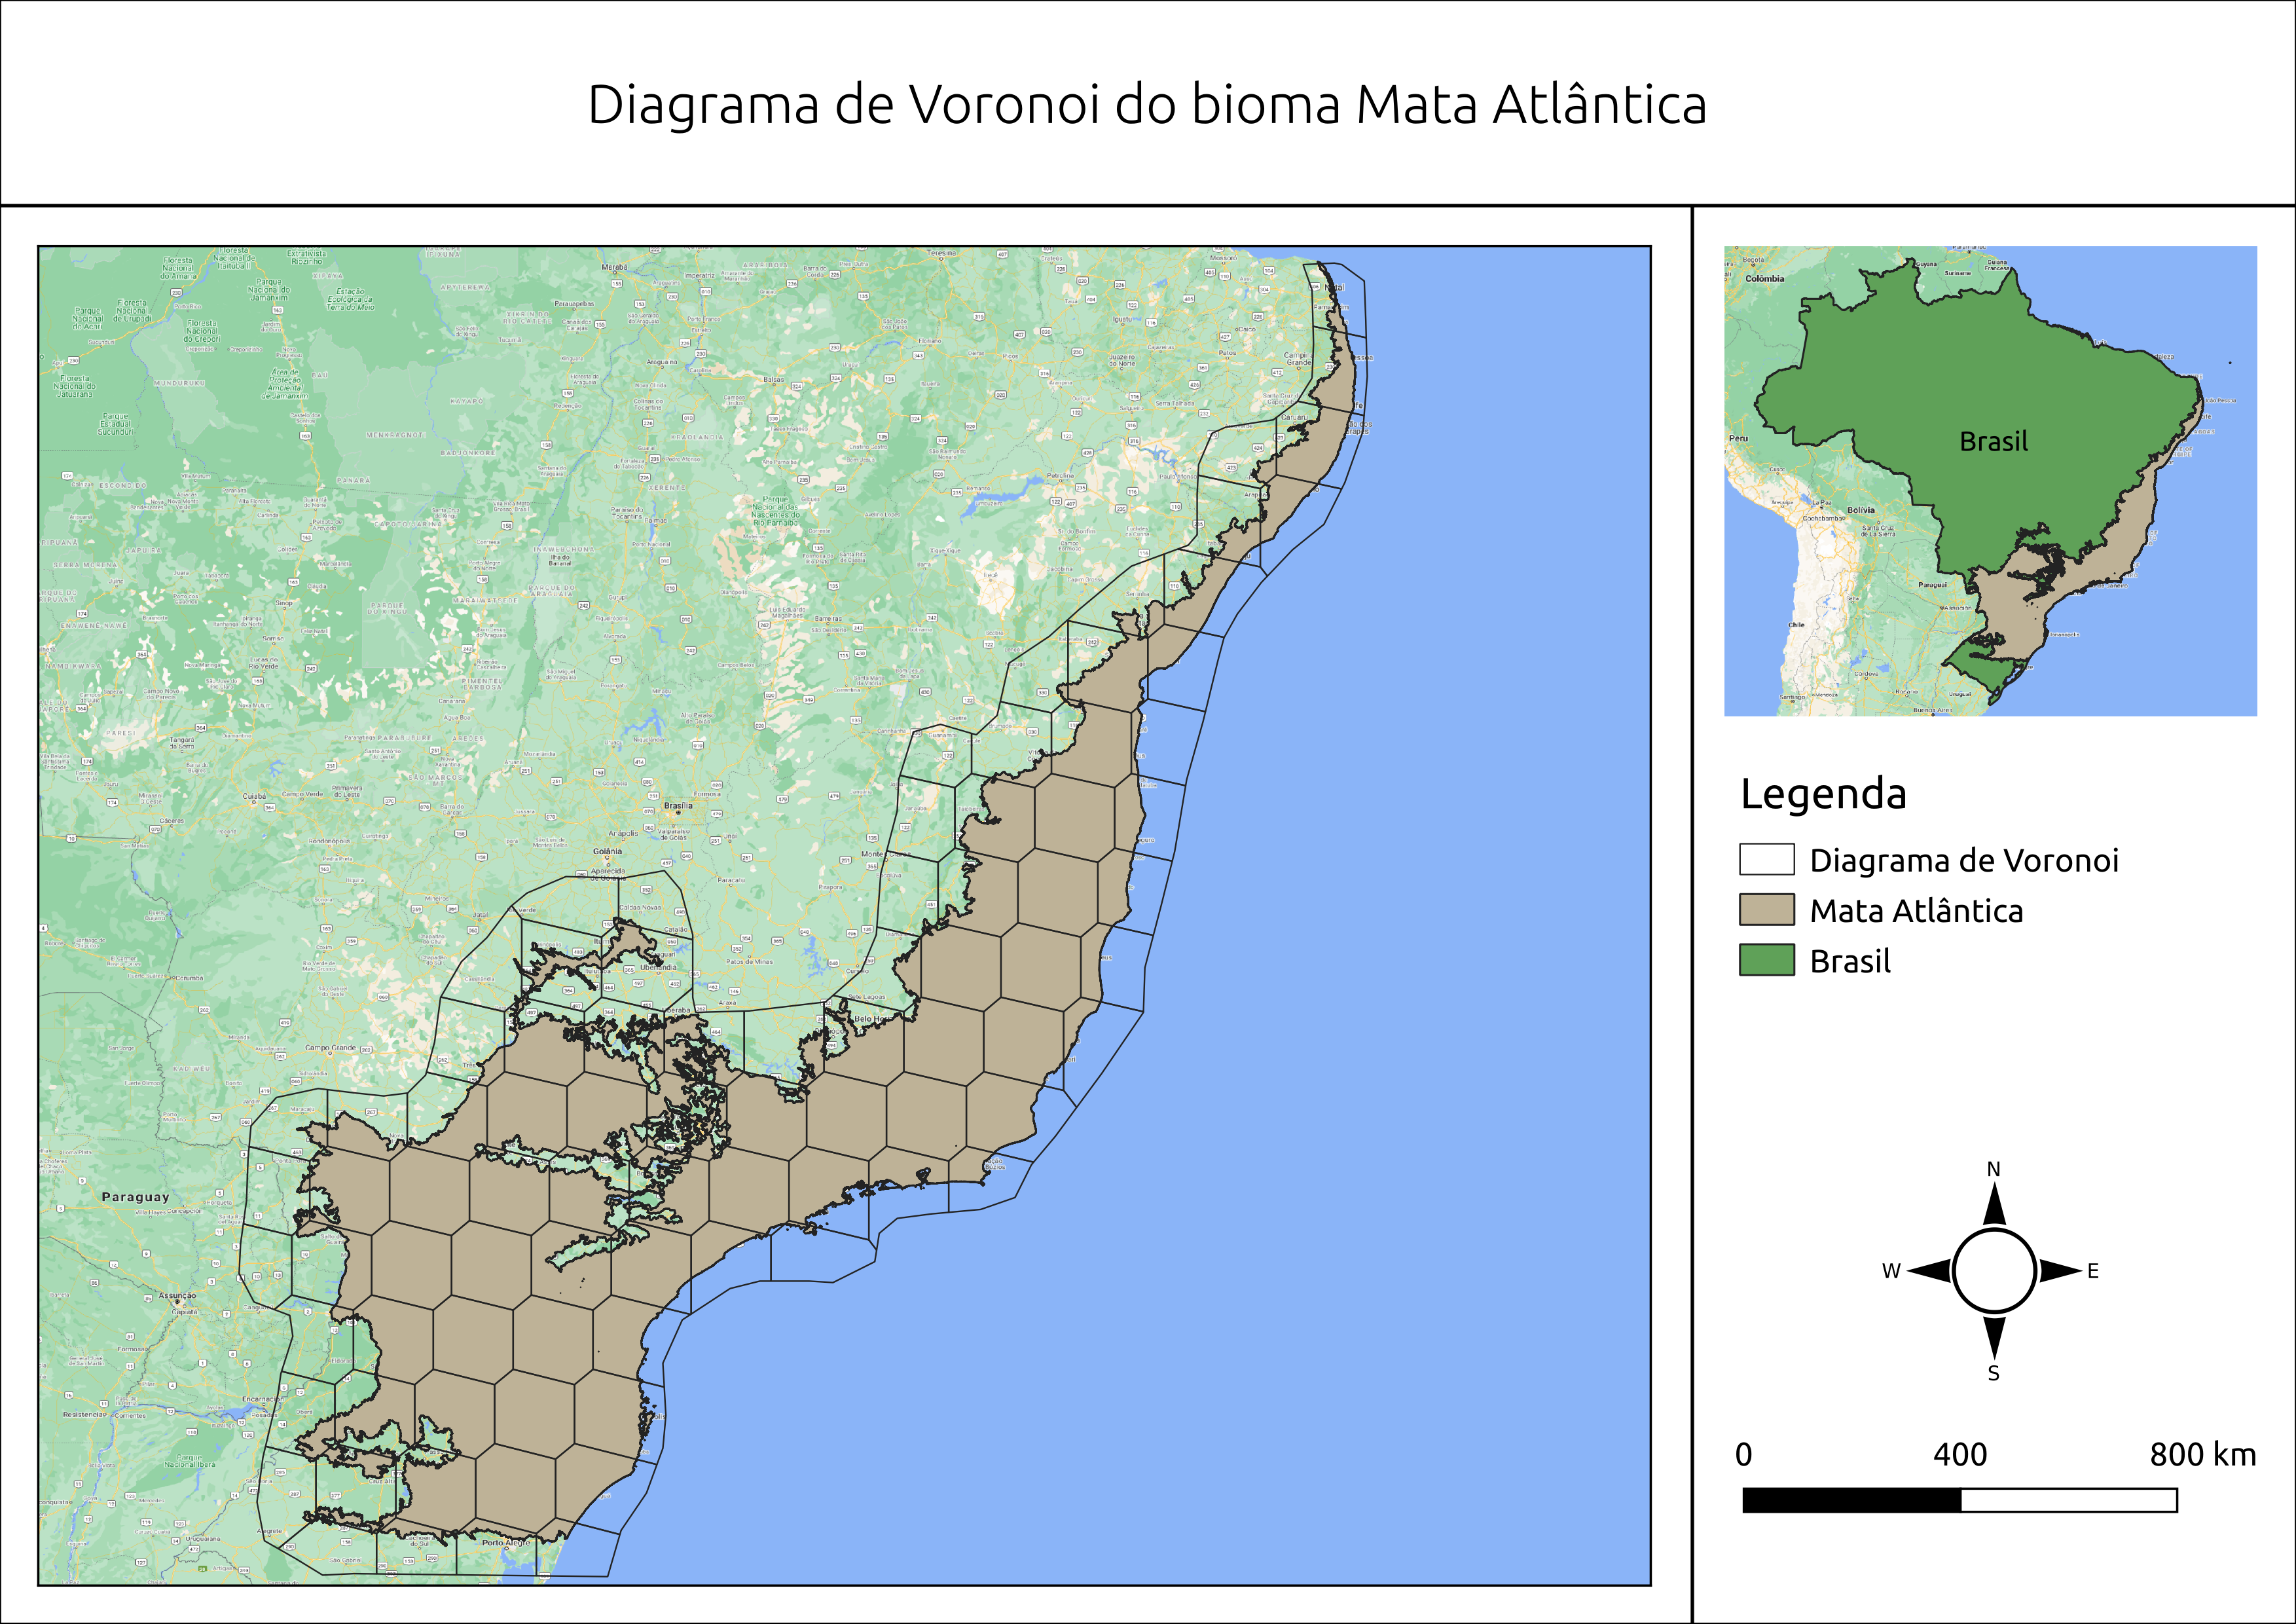
\includegraphics[scale=.5]{images/voronoi_mata_atlantica.png}
    \caption{Diagrama de Voronoi criado a partir dos centróides.}
    \label{fig:voronoi_ma}
\end{figure}

O algoritmo Landtrendr trabalha analisando os valores pixel a pixel para toda a composição de imagens visando criar segmentos e assim identificando trajetórias (Figura \ref{fig:landtrendr_graph}). O Landtrendr pode gerar métricas tanto para distúrbios de perda como de ganho, além de detectar mudanças que ocorreram de forma lenta ou rápida, possibilitando também o cálculo da duração dos eventos segmentados previamente gerando não só dados contínuos como discretos como a duração e o ano da detecção. Podemos analisar, portanto, a história do pixel em questão, neste caso, sob uma perspectiva meso-escalar das florestas de Mata Atlântica. Apesar de receber as bandas padrões do satélite Landsat como dado de entrada, o algoritmo utiliza apenas um único índice para realizar a etapa de segmentação temporal. Alguns índices já bem estabelecidos estão implementados na ferramenta como o NDVI (\textit{Normalized Difference Vegetation Index}), o EVI (\textit{Enhanced vegetation index}), o NDMI (\textit{Normalized Difference Moisture Index}) e o NBR (\textit{Normalized Burn Ratio}). É possível também utilizar uma das próprias bandas do satélite para realizar as análises, como a banda do vermelho ou o SWIR (\textit{Short-wave infrared}). Apesar de bandas como o NBR e NDMI mostrarem bons resultados em regiões de floresta temperada, testes realizados em florestas tropicais mostraram que índices como o NDVI apresentam resultados superiores \citep{zebende2019}. Sendo assim, para este estudo, o processo de segmentação temporal foi realizado utilizando o NDVI como banda base.

\begin{figure}[h!]
    \centering
    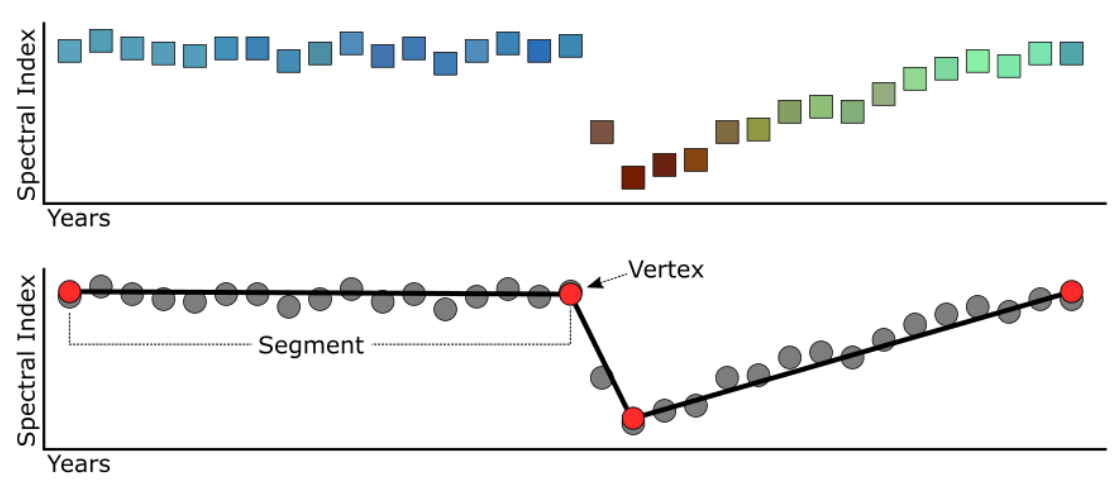
\includegraphics[scale=.8]{images/landtrendr_graphic.png}
    \caption{Segmentação temporal do pixel pelo algoritmo Landtrendr.}
    \label{fig:landtrendr_graph}
\end{figure}

Tanto resultados para o cenário de perda quanto de ganho foram gerados com o objetivo de detectar supressões e processos de degradação como também de restauração e regeneração da floresta. Para este estudo, o Landtrendr foi aplicado utilizando todos seus parâmetros padrões. O tipo de eventos (perda ou ganho) foram organizados de acordo com seu maior evento/segmento (\textit{Greatest Loss / Greatest Gain}).

Toda a etapa de pós-processamento dos dados gerados pelo Landtrendr no GEE foi desenvolvida em ambiente \textit{offline} utilizando ferramentas \textit{open source} como o QGIS \citep{QGIS_software}, GDAL \citep{gdal}, e a linguagem de programação R \citep{Rsoftware} utilizando os pacotes Raster \citep{raster}, Terra \cite{terra}, gdalUtils \citep{gdalutils} e o MLR \citep{mlr}.

\subsubsection{Processamento dos cenários de ganho}

\hspace{13pt} Para o cenário de ganho, todos os parâmetros padrão do algoritmo foram mantidos sem nenhum tipo de restrição. Cenários de magnitude (\textit{magnitude}), valor prévio (\textit{previous value}), ano de detecção (\textit{year of detection}), duração (\textit{duration}) e taxa (\textit{rate}) forma gerados e posteriormente pós-processados para limpeza de ruídos ou para retirada de valores indesejados. 

Primeiramente, foi gerado uma máscara com todas as áreas pseudo-invariantes entre os anos da análise (1985 - 2018) com o intuito de limpar detecções de mudança muito pequenas. Esta máscara representa todos os pixels que não tiveram nenhum tipo de mudança significativa durante todos os anos da análise, ou seja, áreas que em 1985 já eram consideradas floresta e que se mantiveram praticamente iguais até 2018. 

Inicialmente esta máscara foi desenvolvida utilizando composições de imagens Landsat considerando todos os anos da análise e posteriormente classificadas com o algoritmo Random Forest implementado no pacote MLR \citep{mlr}. No entanto, apesar de apresentar resultados promissores quando a aplicada no mapeamento da Bacia Hidrográfica do Rio São João, acabou demonstrando problemas quando extrapolada para o resto do bioma e se mostrou uma técnica altamente custosa tanto em tempo de processamento como no tempo de preparação dos dados. Todo o processo de desenvolvimento desta máscara é detalhada no capítulo 4 deste trabalho. Apesar de não ter sido utilizada como variável neste estudo, a técnica apresentada pode ser de extrema valia quando aplicada em áreas não tão extensas quanto neste caso específico.

Sendo assim, uma nova máscara alternativa teve de ser gerada. Camadas de resultado do projeto Mapbiomas foram utilizadas como uma \textit{proxy}. Todas as imagens classificadas para o bioma foram reclassificadas ano a ano em formato binário (floresta [1] e não-floresta [0]) e posteriormente multiplicadas entre si. Um \textit{raster} final binário foi então gerado, onde os pixels com valor 1 representavam áreas que permaneceram como floresta durante todos os anos do estudo e 0 todos os outros, incluindo todas as outras classes. Esta máscara evitou que muitos eventos pudessem ser classificados como ganho apesar de terem baixa magnitude já que representavam apenas um processo natural nas florestas já existentes. Somente pixels da classe floresta (classe número 3) da série 4.1 foram utilizados. Pixels de classes como floresta plantada foram excluídos assim como o todas as outras.

Além disso, foram mascarados todos os eventos com duração menor ou igual a 4 anos, já que não gostaríamos de incorporar eventos ainda muito recentes que poderiam ser identificados como falsos eventos de mudança. O valor mínimo de 5 anos para eventos de ganho ajuda a identificar apenas eventos mais longos que tiveram tempo de apresentar respostas espectrais significativas de recuperação. Com 5 anos a vegetação já passa a apresentar um estágio sucessional característico de floresta secundária inicial \citep{Chazdon2014}. 

\subsubsection{Processamento dos cenários de perda}
\hspace{13pt} Assim como o cenário de ganho, o processamento do cenário de perda utilizou todos os parâmetros padrões do algoritmo sem nenhum tipo de restrição com o objetivo de realizar limpezas nos resultados obtidos apenas em uma etapa de pós-processamento. Os mesmos cenários de magnitude (\textit{magnitude}), valor prévio (\textit{previous value}), ano de detecção (\textit{year of detection}), duração (\textit{duration}) e taxa (\textit{rate}) forma gerados.

No caso das perdas, criou-se uma máscara para garantir que o Landtrendr fosse capaz de detecção mudanças de perda apenas em áreas que foram classificadas como floresta pelo projeto Mapbiomas no ano de 1985. Essa máscara ajuda na não seleção de áreas que nem mesmo eram classificadas como florestas mas que sofreram algum tipo de perda com magnitude grande o suficiente para ser detectada pelo algoritmo. Além disso, uma outra máscara foi gerada, para excluir áreas que apesar de terem sido mapeadas em 1985 como floresta e terem sofrido algum tipo de perda significativa, sofreram algum processo de restauração ou regeneração natural ao longo dos anos. Sendo assim, o resultado final para o dado de perdas visou somente a seleção de áreas que tiveram floresta, que perderam essa vegetação e que não apresentaram nenhum processo de recuperação significativa.

Diferentemente dos dados de ganho, os dados de perda tem como característica importante a grande variabilidade na duração dos eventos. Sendo assim, utilizou-se a camada de duração para gerar, além das camadas de perda gerais, camadas de perda com duração igual a um ano e camadas com duração superior à um ano. Esta diferenciação é importante para que possamos identificar eventos de perda rápida, sejam eles de natureza antrópica ou natural, normalmente associados à cortes rasos ou queimadas. 

% \subsubsection{Validação}

\subsection{Resultados e Discussões}

\hspace{13pt} Os resultados para os cenários de perda e ganho foram agregados para abranger em um único arquivo todo o bioma. Com isso, foi possível com compilar os resultados transformando os arquivos matriciais em arquivos vetoriais. Essa transformação foi necessária para facilitar a visualização através de mapas de calor (\textit{heatmaps}) como os que veremos posteriormente. Os resultados foram transformados para um sistema de referência de área igual ideal para grandes extensões. Neste caso foi utilizado a projeção de Albers, mais especificamente a \textit{South America Albers Equal Area Conic} (ESRI: 102003). 

\subsubsection{Os eventos de perda na Mata Atlântica}

\hspace{13pt} Somando-se todos os eventos de perda detectados pelo algoritmo após as filtragens necessárias, houveram ao longo de todos os anos da análise 61.167.796 de pixels com uma perda média de magnitude de 225 ou diminuição de 0.225 no índice NDVI. Isso equivale a uma área total de pouco mais de 55 mil $ km^2 $ de florestas que sofreram perdas significativas no bioma e que não foram recuperadas após a supressão.

De forma geral, pode se dizer que um evento de perda com magnitude igual ou superior a 200 tem alta probabilidade de ser considerado um evento de perda significativa a ponto de representar uma mudança estrutural na cobertura da terra e uma consequente mudança de classe em mapas de uso e cobertura. Este número foi encontrado através de testes estatísticos realizados com o intuito de entender diferenças espectrais entre áreas de floresta e pasto utilizando o índice NDVI como base. 

Os testes foram realizados tanto para áreas de florestas ombrófilas quanto estacionárias por representarem as duas maiores fitofisionomias encontradas no bioma. Cem amostras foram coletadas para cada fitofisionomia de floresta como também para áreas de pasto. O valor médio de NDVI encontrado para áreas de floresta estacionária foi de 0.80 e ombrófila de 0.86. Já para áreas de pasto o valor médio foi de 0.61. Ou seja, uma diferença média de mais de 0.2 ou mais de 200 de magnitude entre áreas florestadas e de pasto. Comparando-se as médias das amostras de floresta ombrófila com amostras de pasto o p-valor obtido foi de 1.599e-11, já para a comparação com as amostras de florestas estacionárias o valor do teste-t foi de 2.495e-7. Ou seja, independente da fitofisionomia, ambas as situações apresentaram diferença estatisticamente significativa em suas médias.

No entanto, este valor de limiar encontrado não foi utilizado como máscara para as análises de perda devido a um alto desvio padrão encontrado nos valores de magnitude (média de 123). Foi observado que muitas áreas que já apresentavam um certo grau de degradação já faziam a transição para pasto com evento de magnitude próximas de 150. Para não excluirmos estas áreas do resultado, optou-se por utilizar apenas máscaras baseadas em camadas previamente geradas pelo projeto Mapbiomas como descrito na sessão 3.2.5.

O resultado mais abrangente envolvendo todos os eventos de perda do bioma pode ser visualizado na (Figura \ref{fig:heat_loss_masked85_maskedgain}). A maior aglomeração de eventos de perda está localizada principalmente entre os estados do Paraná e Santa Catarina e no estado da Bahia. Nos outros estados o mapa de calor mostra uma distribuição mais homogênea dos eventos ao longo do território. 

\begin{figure}[H]
    \centering
    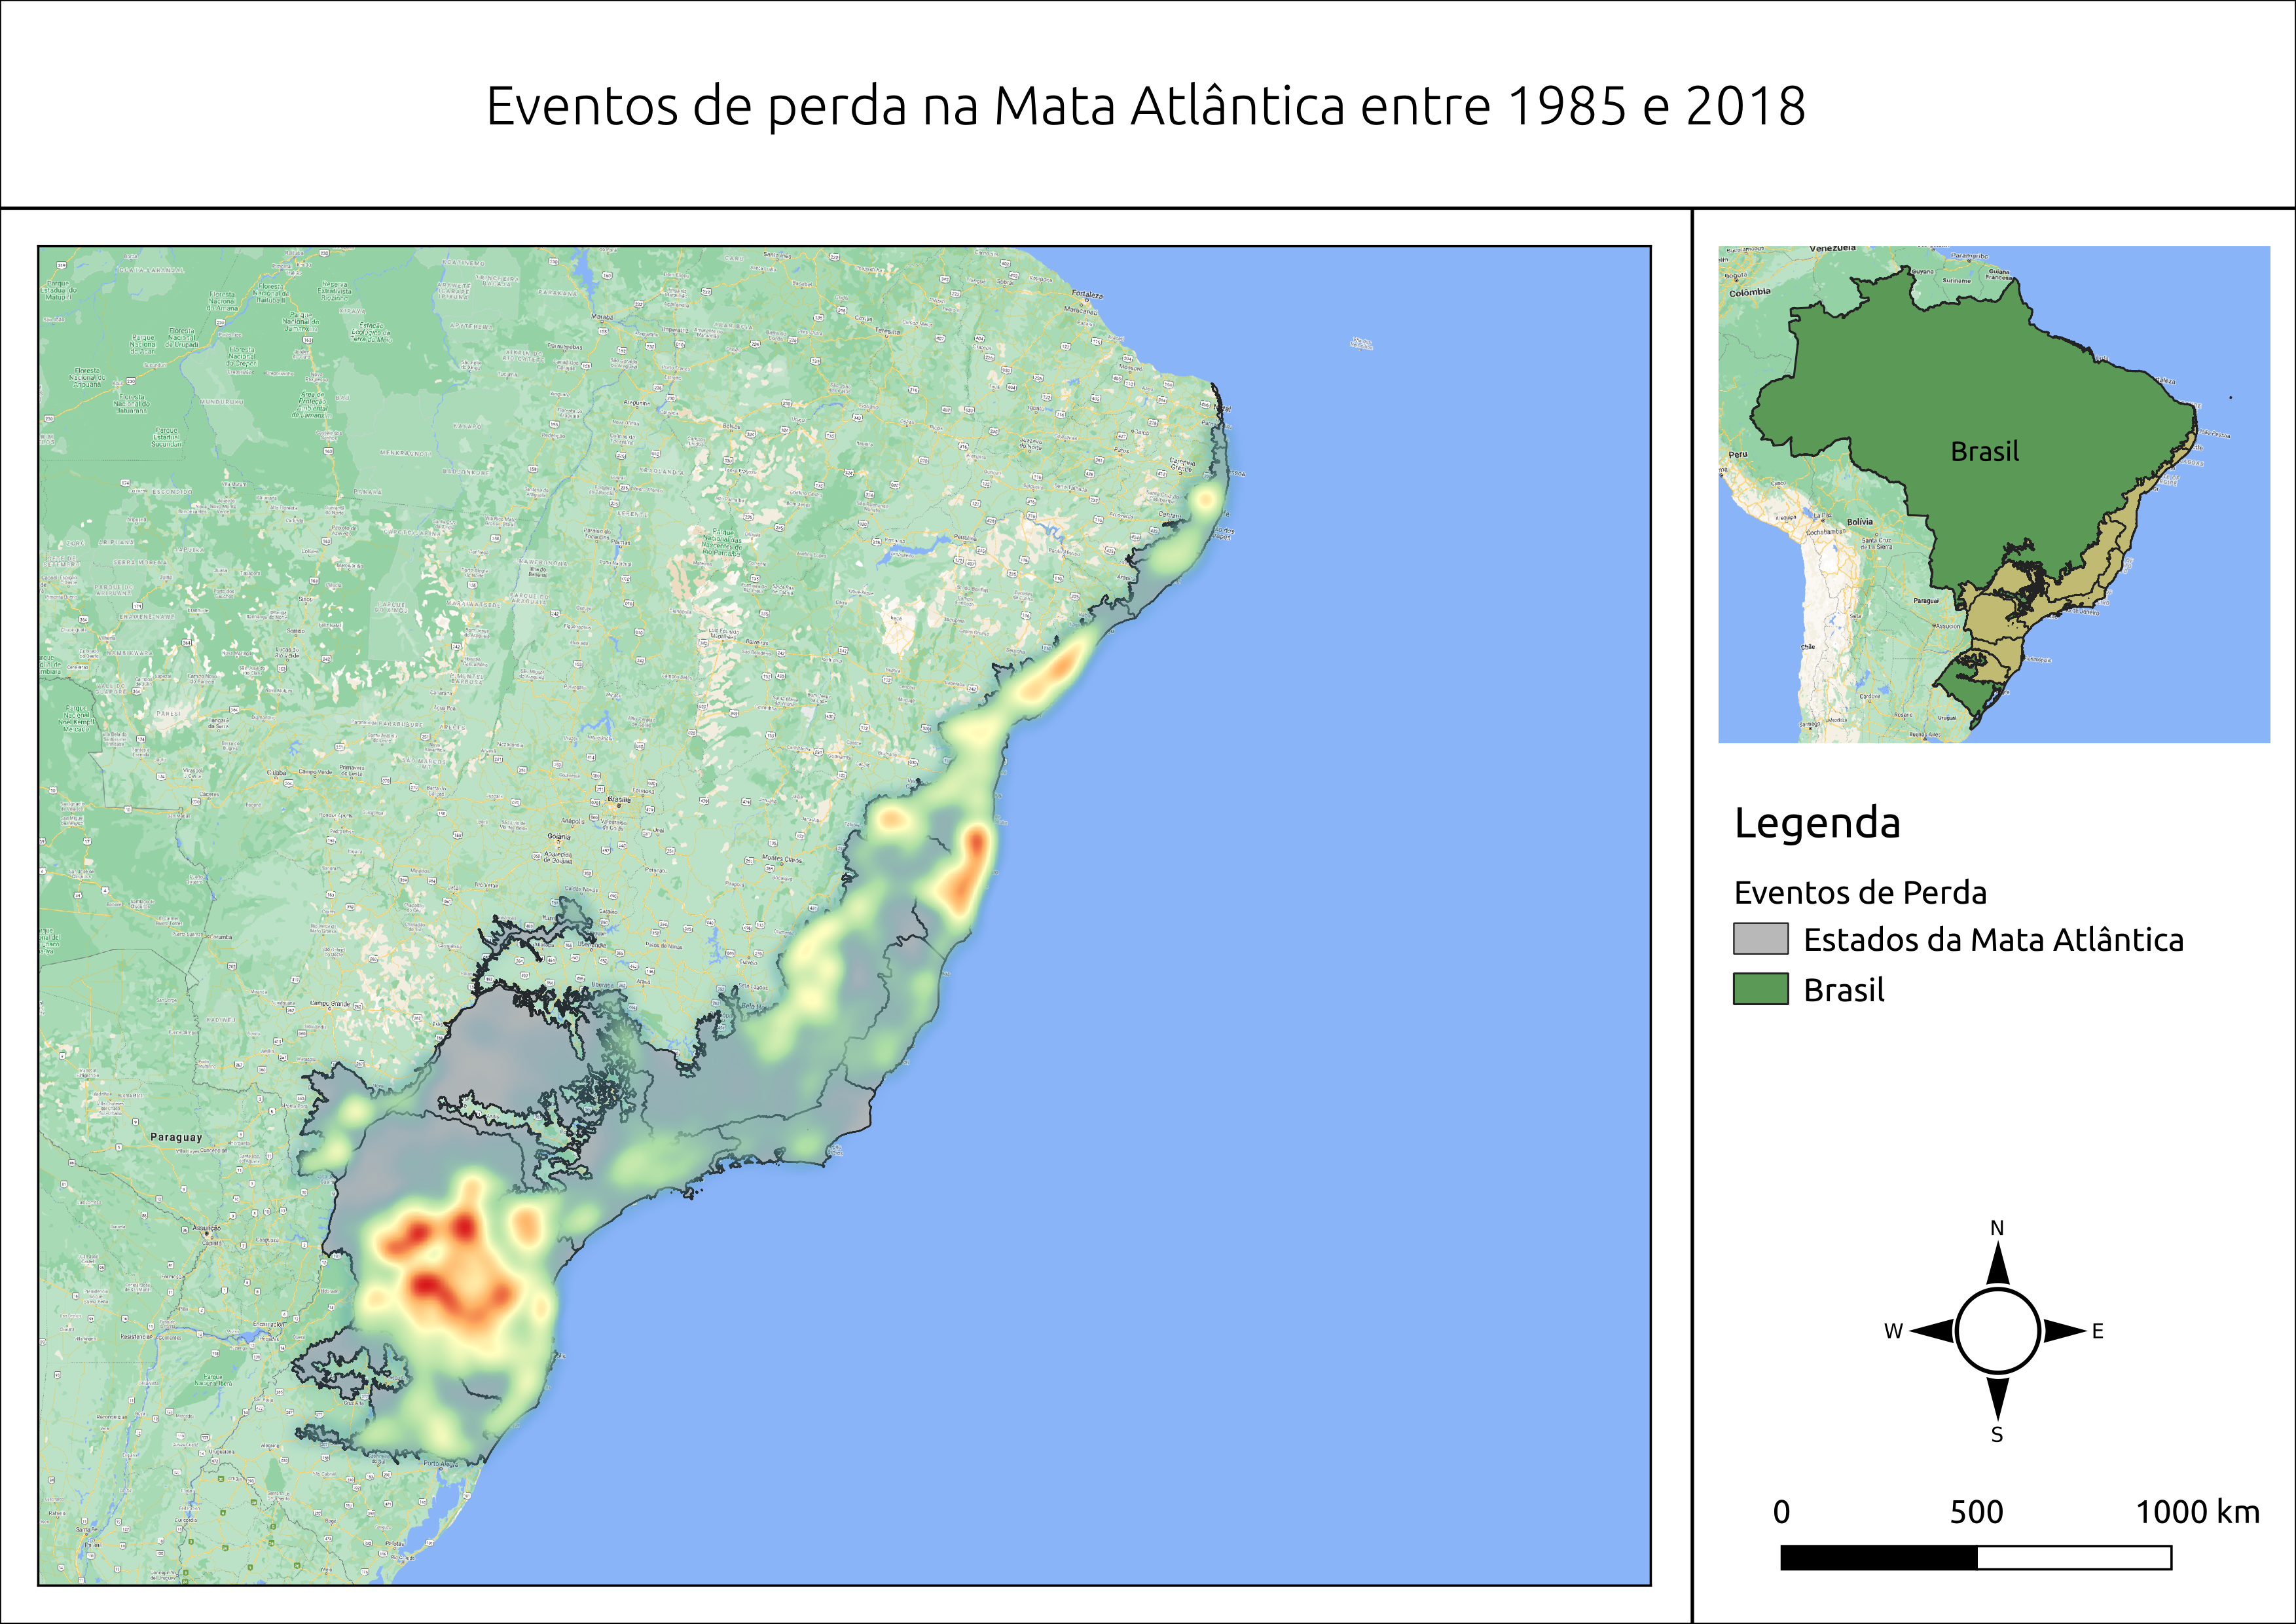
\includegraphics[scale=.5]{images/heatmap_loss_masked85_maskedgain.png}
    \caption{Todos os eventos de perda na Mata Atlântica entre 1985 e 2018.}
    \label{fig:heat_loss_masked85_maskedgain}
\end{figure}

Quando a divisão das detecções é feita de acordo com eventos de curta duração (um ano) e longos (maiores que um ano), verificamos que o padrão espacial das aglomerações (\textit{clusters}) se mantém semelhante com apenas algumas variações (Figura \ref{fig:heat_loss_eq1_neq1}). Os eventos de curta duração tendem a se localizar mais na fronteira entre Paraná e Santa Catarina, enquanto os de longa aconteceram com maior frequência na região central do Paraná, sul/norte da Bahia e norte de Pernambuco. Dos mais de 61 milhões de eventos detectados ou 55 mil $ km^2 $, cerca de 27.5 milhões foram eventos de curta duração, o que significa uma área aproximada de 25 mil $ km^2 $. Os outros 33.7 milhões de eventos tiveram duração maior que um ano, o que totalizou aproximadamente 30.4 mil $ km^2 $.

Já quando a divisão é feita por estados (Figura \ref{fig:estados_loss_masked85_maskedgain}), verificamos que estados como Minas Gerais possuem um número grande de eventos que estão distribuídos de forma homogênea pelo território, assim como Bahia e São Paulo. Vemos que apesar do maior \textit{cluster} de perdas estar localizado entre Paraná e Santa Catarina, a maior quantidade de eventos está no estado do Paraná. 

\begin{figure}[H]
    \centering
    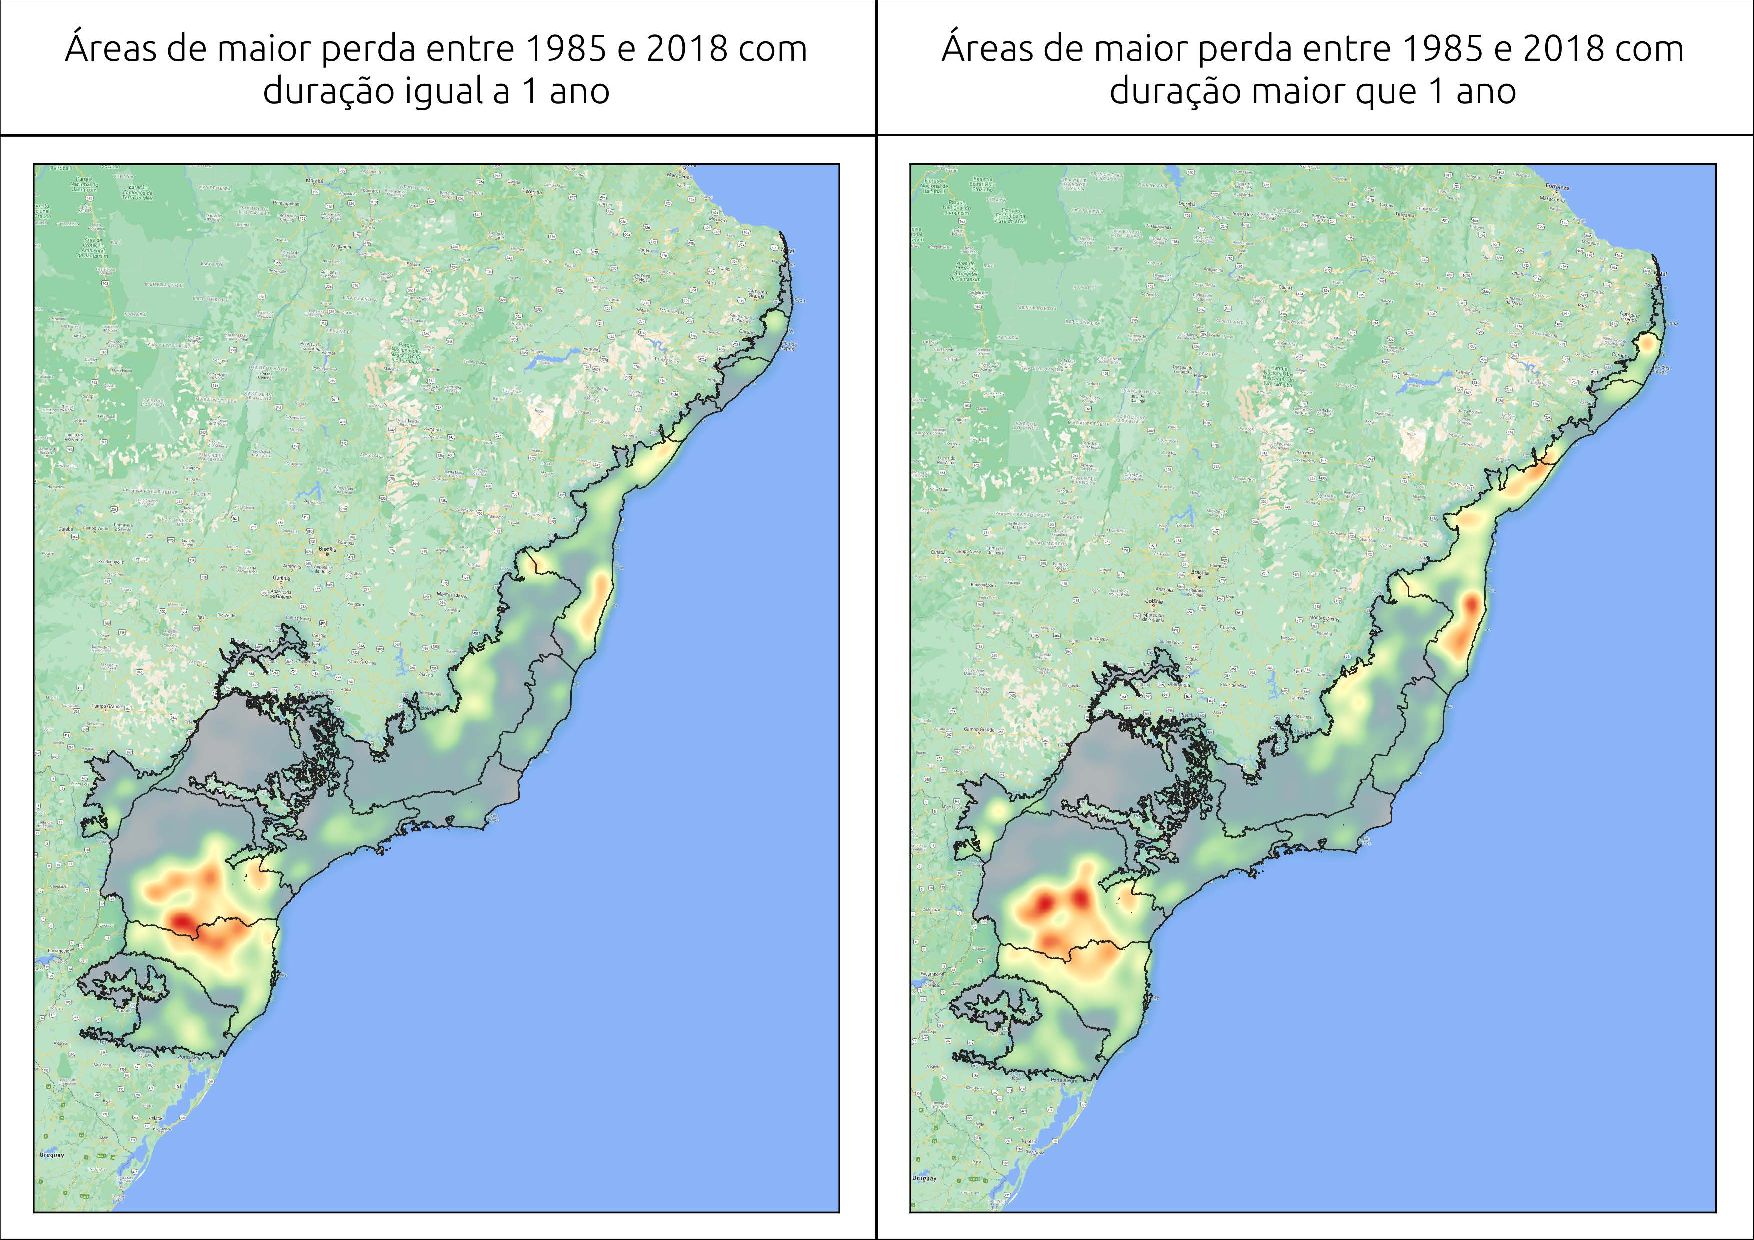
\includegraphics[scale=.5]{images/heatmap_loss_eq1_neq1.png}
    \caption{Mapas com os eventos de perda entre 1985 e 2018 tanto com duração igual a 1 quanto somente maiores que 1.}
    \label{fig:heat_loss_eq1_neq1}
\end{figure}

\begin{figure}[H]
    \centering
    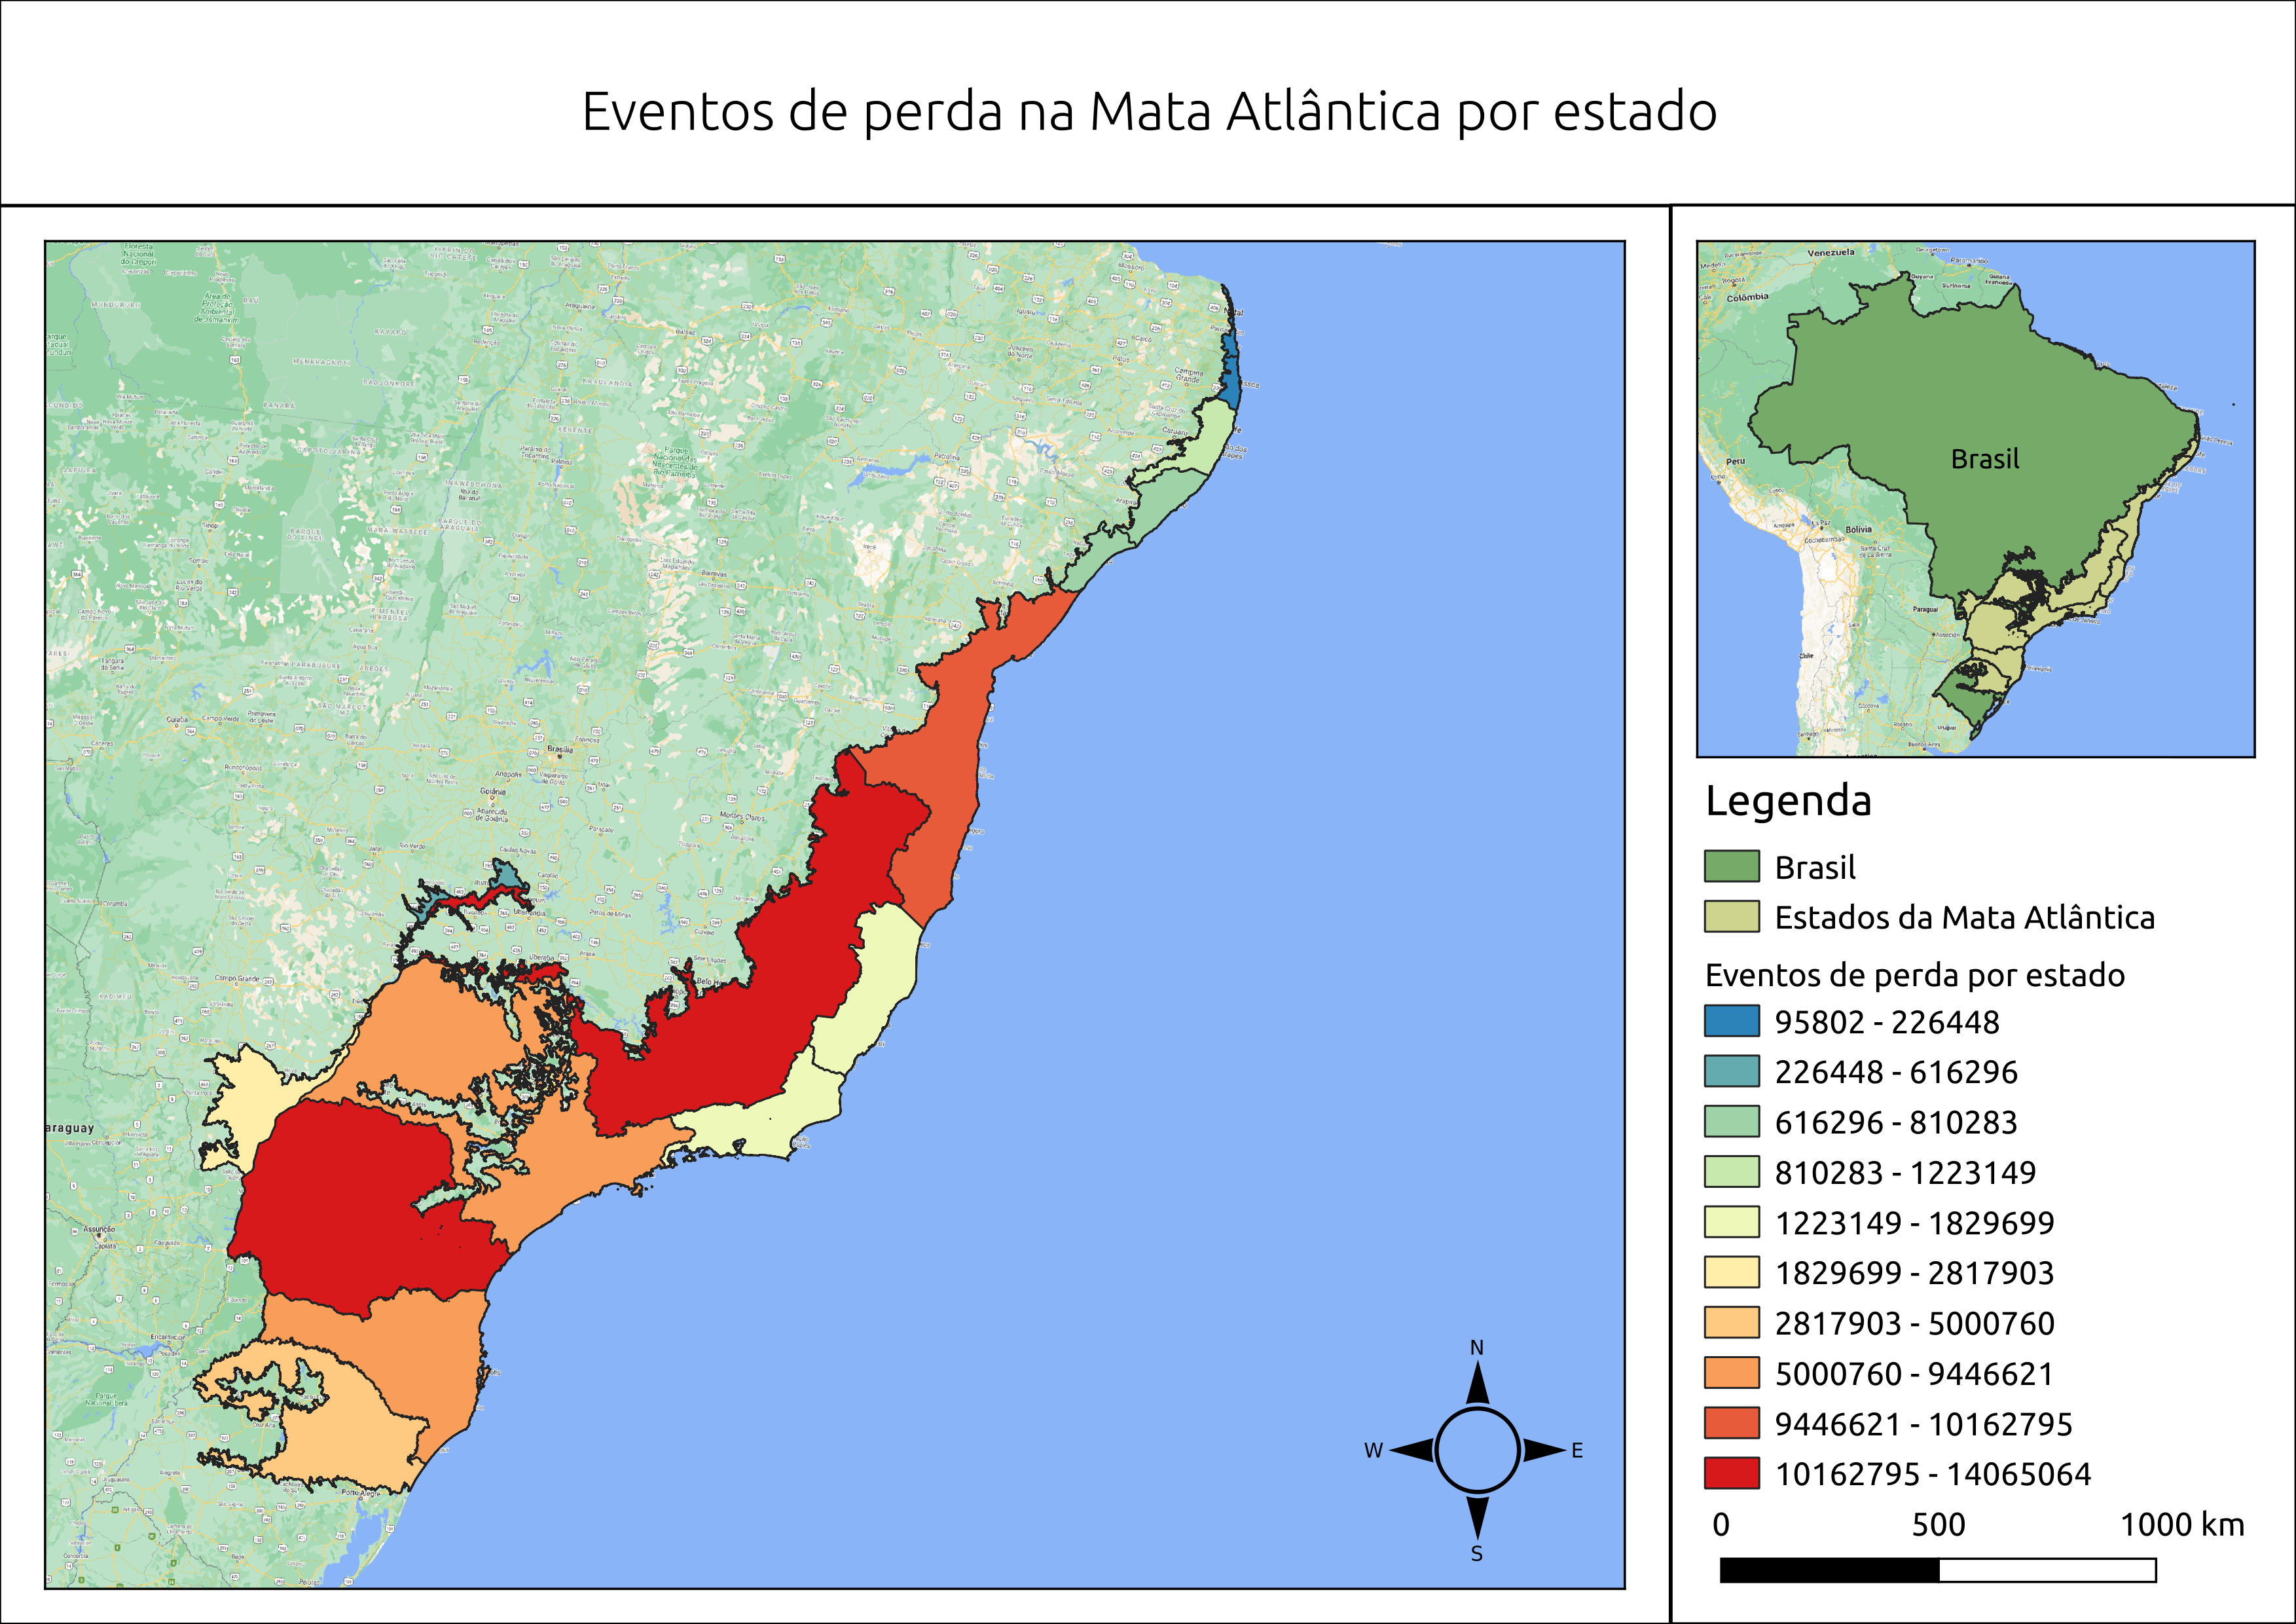
\includegraphics[scale=.5]{images/estados_loss_masked85_maskedGain.png}
    \caption{Todos os eventos de perda na Mata Atlântica entre 1985 e 2018 por estado. Os valores representam o número de pixels que tiveram alguma detecção de perda.}
    \label{fig:estados_loss_masked85_maskedgain}
\end{figure}

Ao considerar o número de eventos de acordo com a área de cada estado, verificamos que estados como Santa Catarina e Bahia se destacam mostrando o maior proporção de perdas ao longo dos 33 anos seguido de Pernambuco, Paraná e Sergipe (Figura \ref{fig:estados_loss_proporcional}).

\begin{figure}[H]
    \centering
    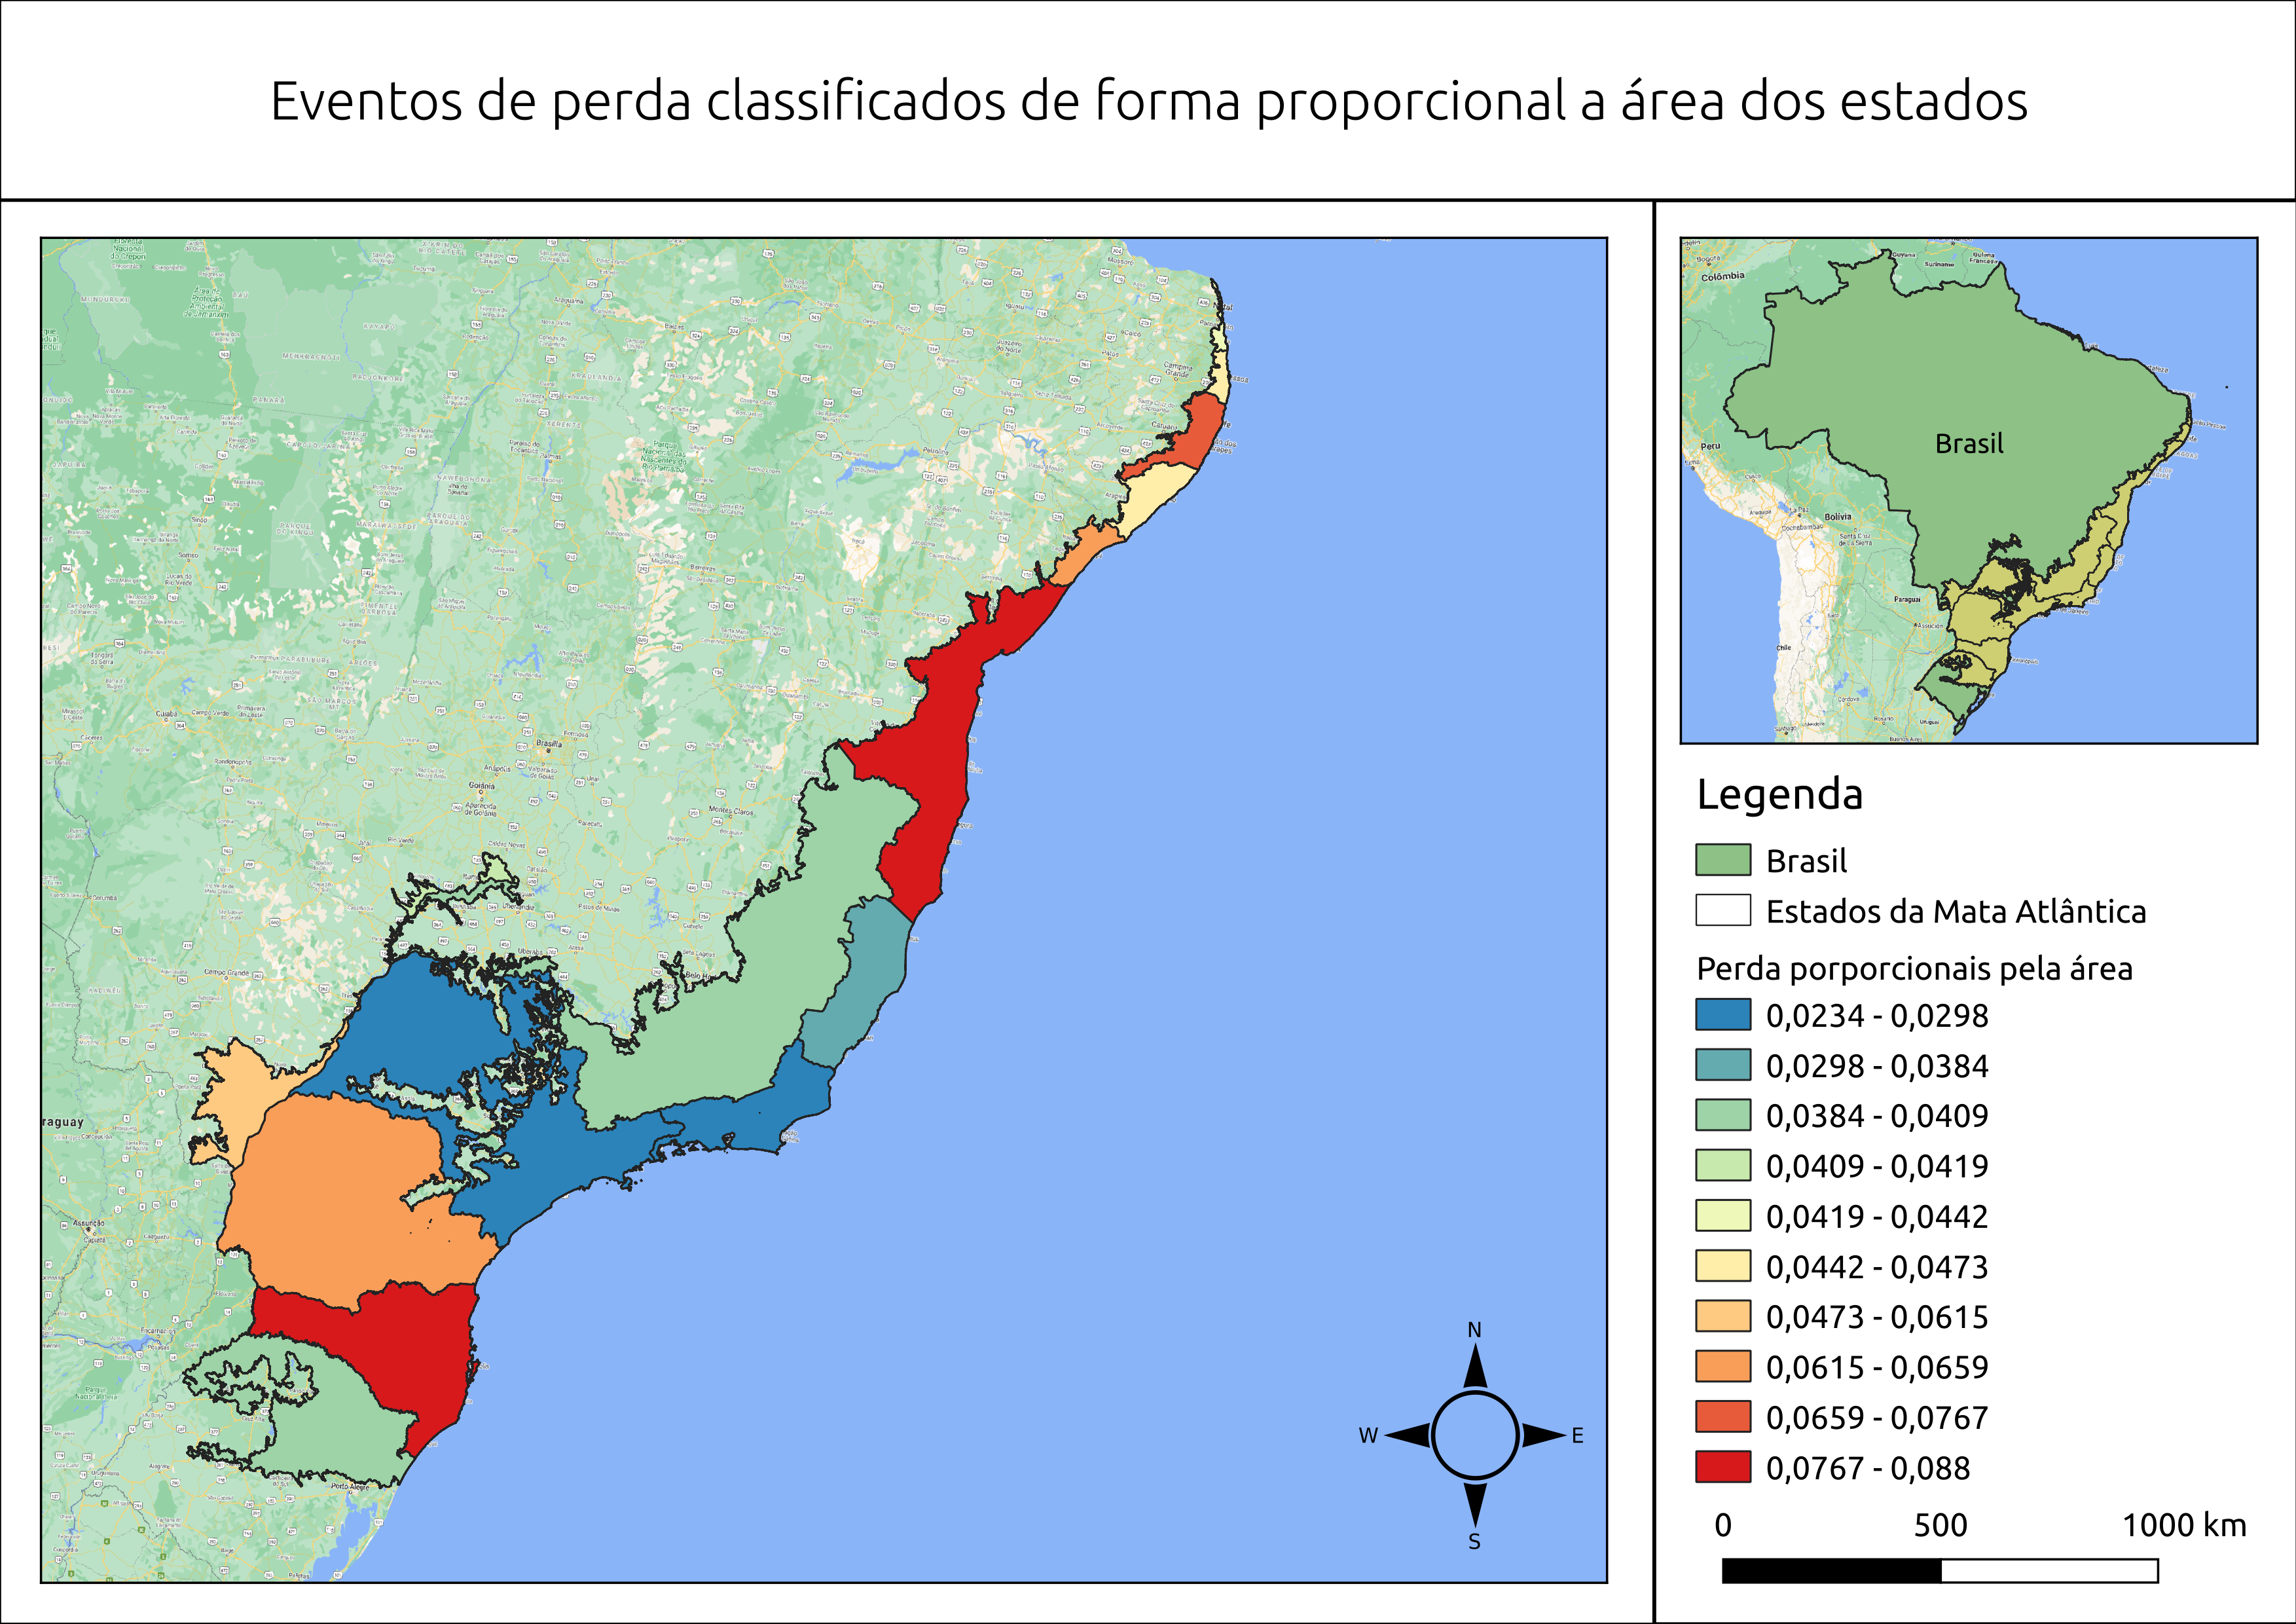
\includegraphics[scale=.5]{images/estado_loss_proporcional.png}
    \caption{Mapas com os eventos de perda entre 1985 e 2018 classificado de acordo com a proporção de área de cada estado.}
    \label{fig:estados_loss_proporcional}
\end{figure}

Como visto previamente no mapa de \textit{clusters}, os eventos de perda de curta duração tendem a se concentrar principalmente no Paraná e Santa Catarina quando analisados sob divisões políticas (Figura \ref{fig:estados_loss_masked85_maskedgain_eq1}). Já os de longa duração, se concentram em estados como o Paraná e Bahia, seguido de Minas Gerais, Santa Catarina e São Paulo (Figura \ref{fig:estados_loss_masked85_maskedgain_neq1}).

Quando realizamos a divisão por municípios (Figura \ref{fig:mun_loss_masked85_maskedgain}), o padrão espacial similar ao \textit{heatmap} da Figura \ref{fig:heat_loss_masked85_maskedgain}, mas demonstra como eventos que anteriormente estavam aparentemente distribuídos de forma mais homogênea, se agrupam quando classificados por município. As aglomerações ainda permanecem ocorrendo principalmente em estados como Paraná, Santa Catarina e Bahia, mas podemos observar municípios em outros estados que concentraram um maior número de perda como em Iguatemi no Mato Grosso do Sul ou em Águas Vermelhas em Minas Gerais. A lista completa com todos os 3078 municípios pertencentes ao bioma pode ser acessado neste link \url{https://github.com/sacridini/municipios_perdas_ganhos}.

\begin{table}[h!]
    \centering
    \rowcolors{2}{red!50!yellow!30}{green!40!yellow!10}
    % \footnotesize
    \begin{tabular}{|c | c | c|}
    \hline
                    Nome & Eventos & UF \\
            Porto Seguro & 444892 & BA \\
           Prudentópolis & 425340 & PR \\
              Ortigueira & 373635 & PR \\
 Coronel Domingos Soares & 367051 & PR \\
                Belmonte & 333728 & BA \\
               Itamaraju & 329167 & BA \\
              Guarapuava & 314087 & PR \\
     Santa Cruz Cabrália & 296493 & BA \\
                   Prado & 283573 & BA \\
             Canavieiras & 279240 & BA \\
    Rio Bonito do Iguaçu & 271232 & PR \\
                  Pinhão & 270471 & PR \\
            Encruzilhada & 264281 & BA \\
                 Reserva & 263798 & PR \\
                Bituruna & 262246 & PR \\
                  Tibagi & 253448 & PR \\
                   Mafra & 251392 & SC \\
           Santa Cecília & 246603 & SC \\
              Itaiópolis & 246205 & SC \\
              Guaratinga & 241392 & BA \\
    \hline
    \end{tabular}
    \caption{Os vinte municípios com maior número de eventos de perda}
    \label{tab:mun_loss}
\end{table}

\begin{figure}[H]
    \centering
    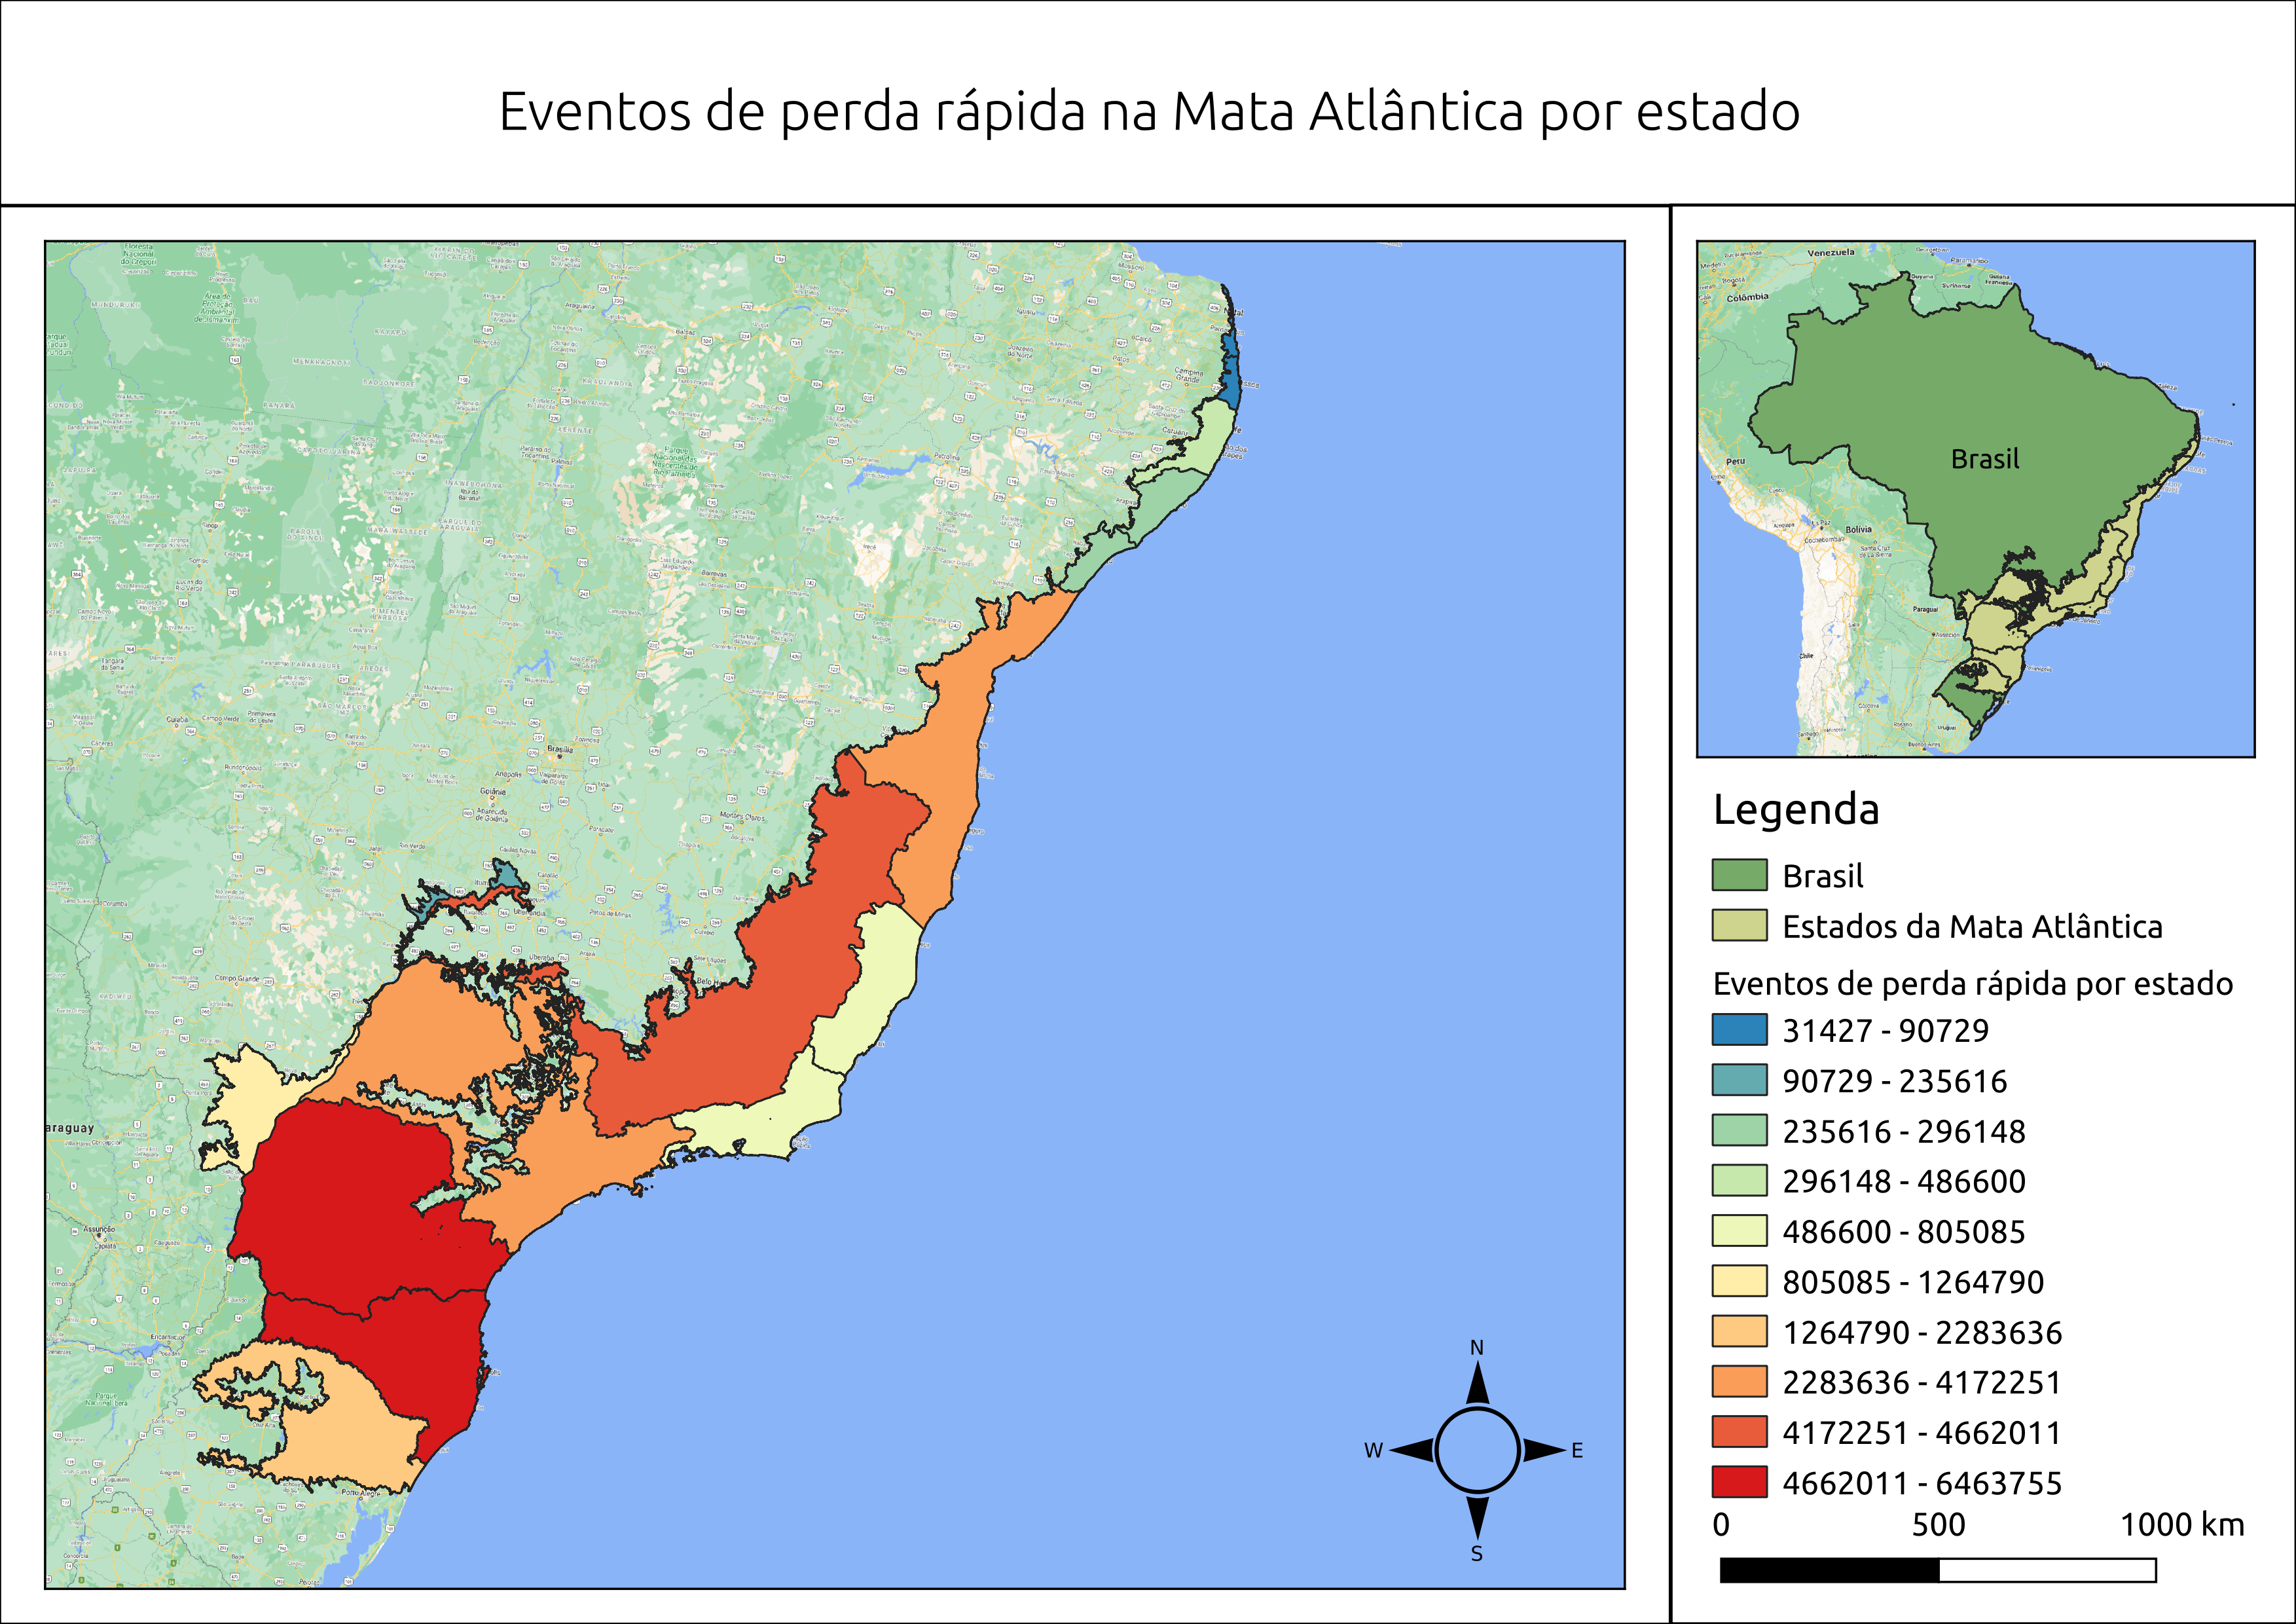
\includegraphics[scale=.5]{images/estados_loss_masked85_maskedGain_eq1.png}
    \caption{Todos os eventos de perda rápida (duração igual a 1) na Mata Atlântica entre 1985 e 2018 por estado. Os valores representam o número de pixels que tiveram alguma detecção de perda.}
    \label{fig:estados_loss_masked85_maskedgain_eq1}
\end{figure}

\begin{figure}[H]
    \centering
    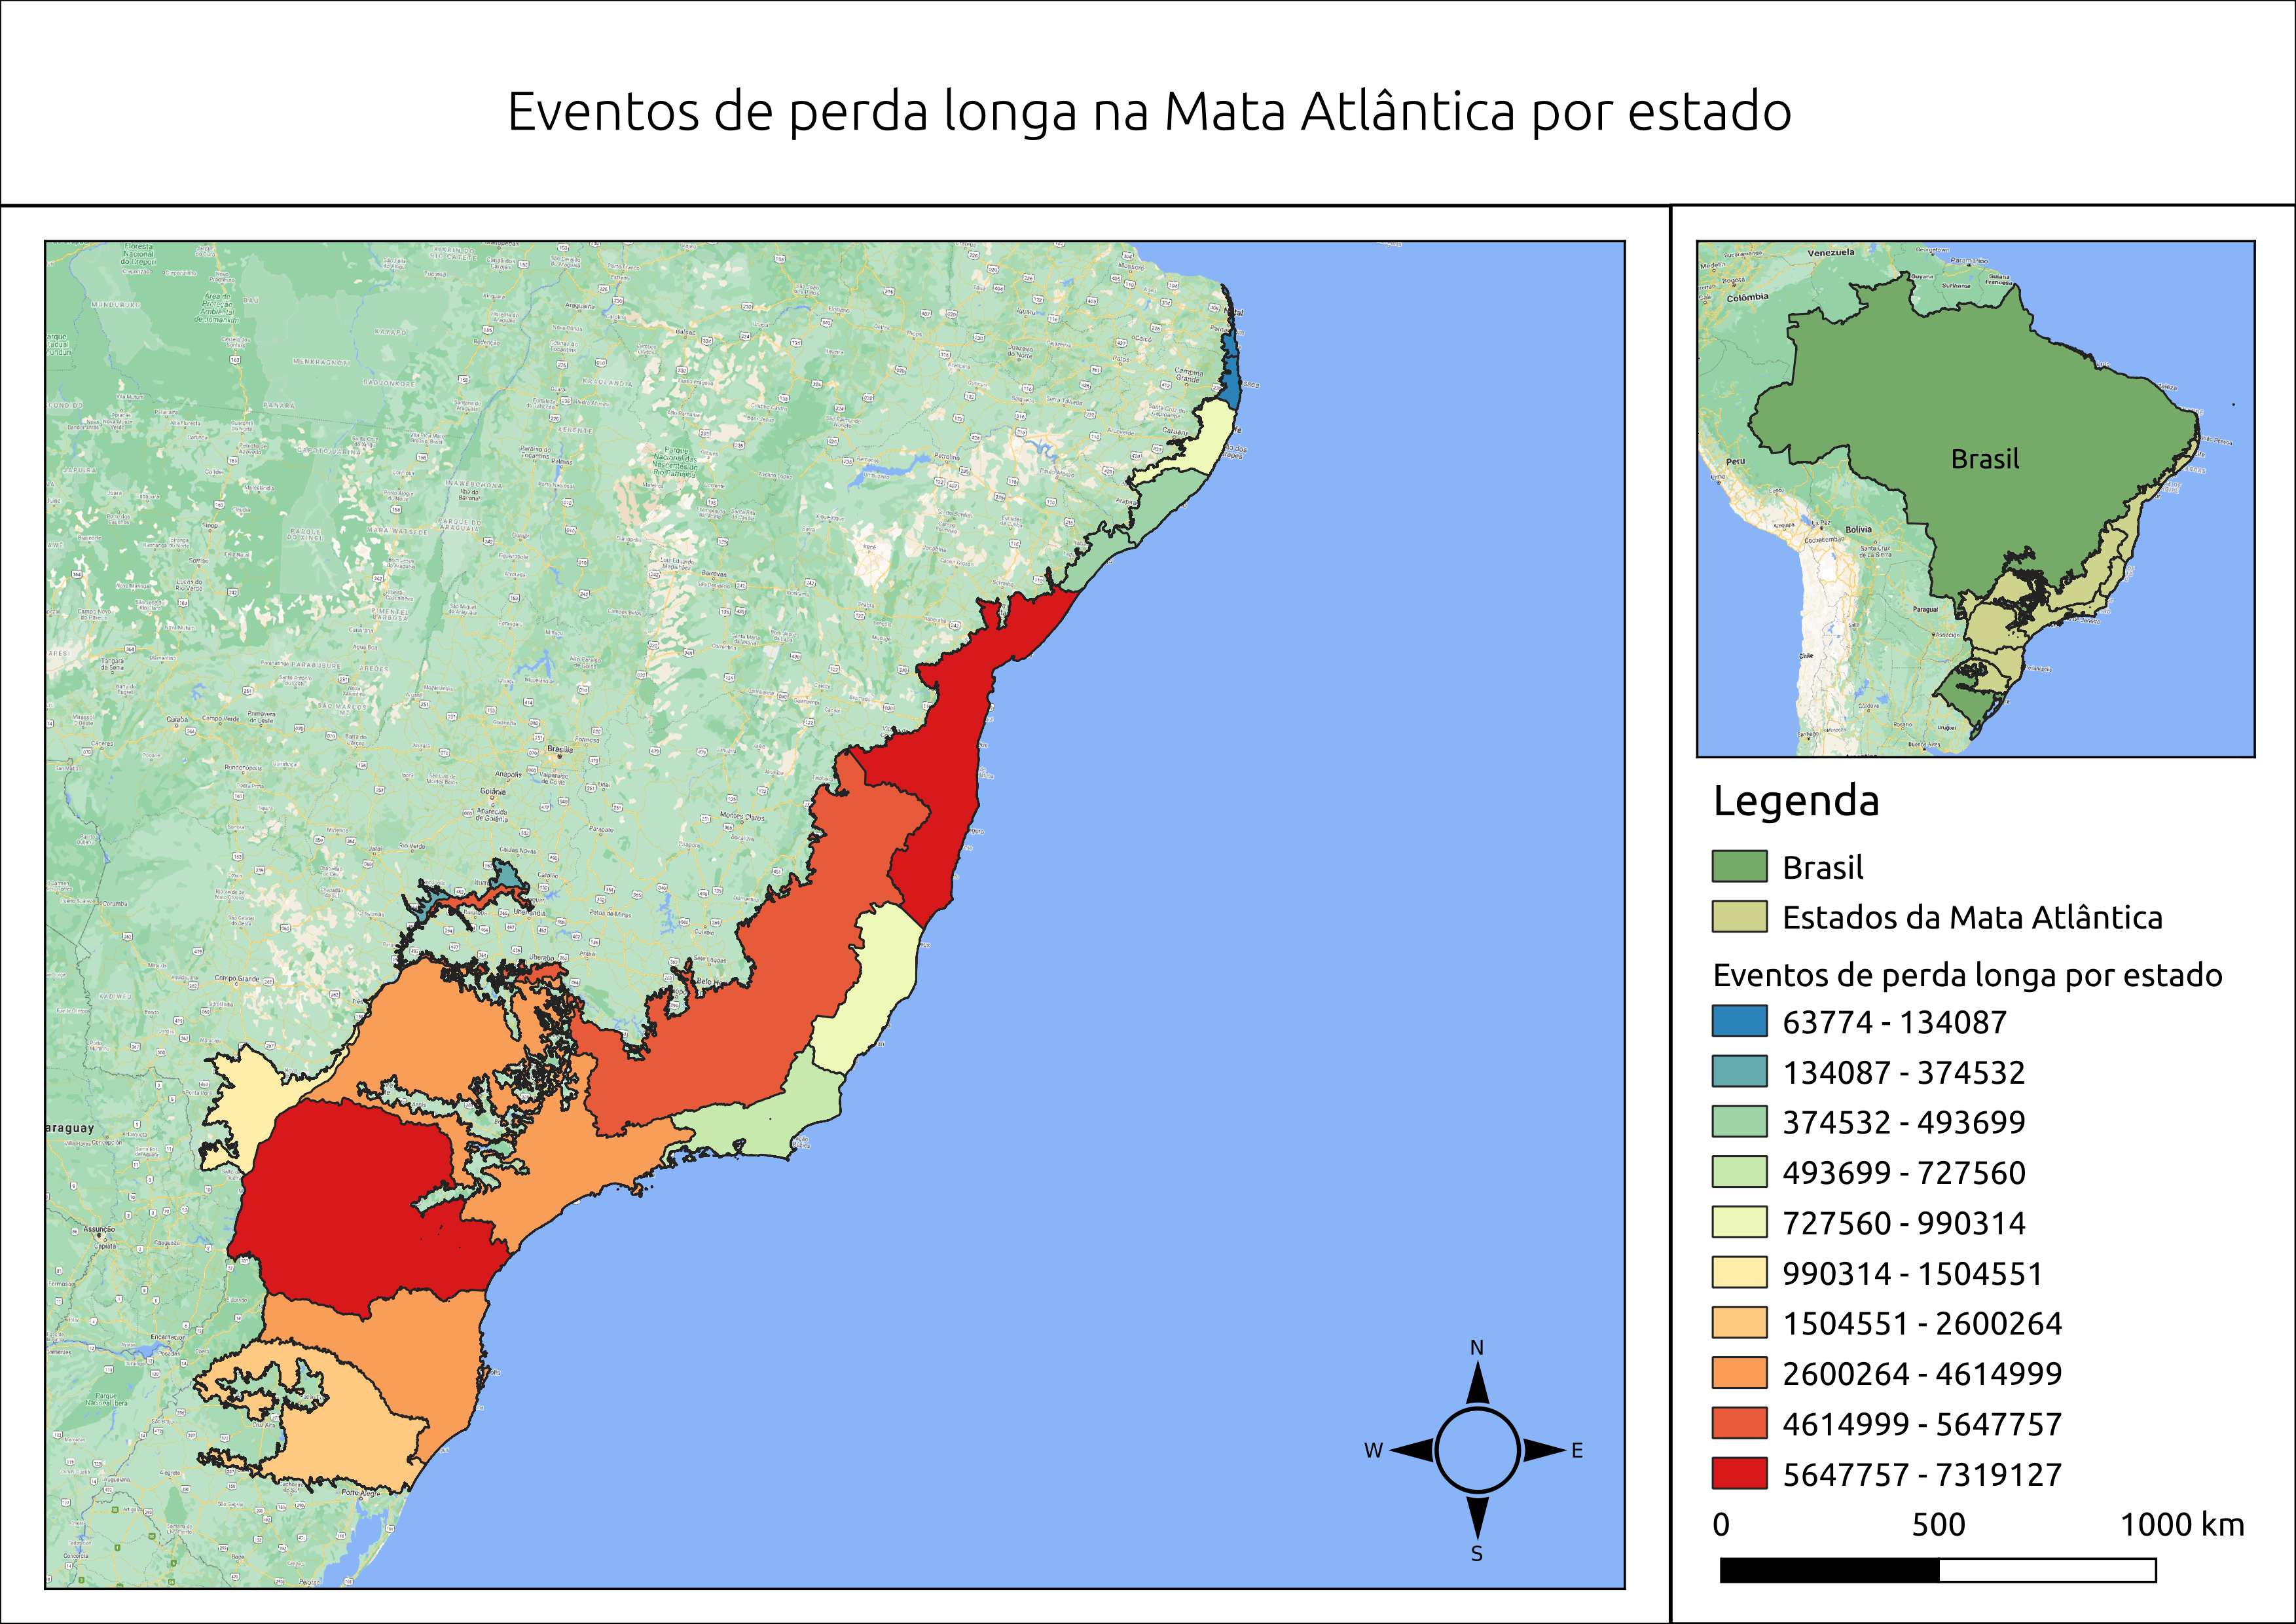
\includegraphics[scale=.5]{images/estados_loss_masked85_maskedGain_neq1.png}
    \caption{Todos os eventos de perda longa (duração maior que 1) na Mata Atlântica entre 1985 e 2018 por estado.}
    \label{fig:estados_loss_masked85_maskedgain_neq1}
\end{figure}

\begin{figure}[H]
    \centering
    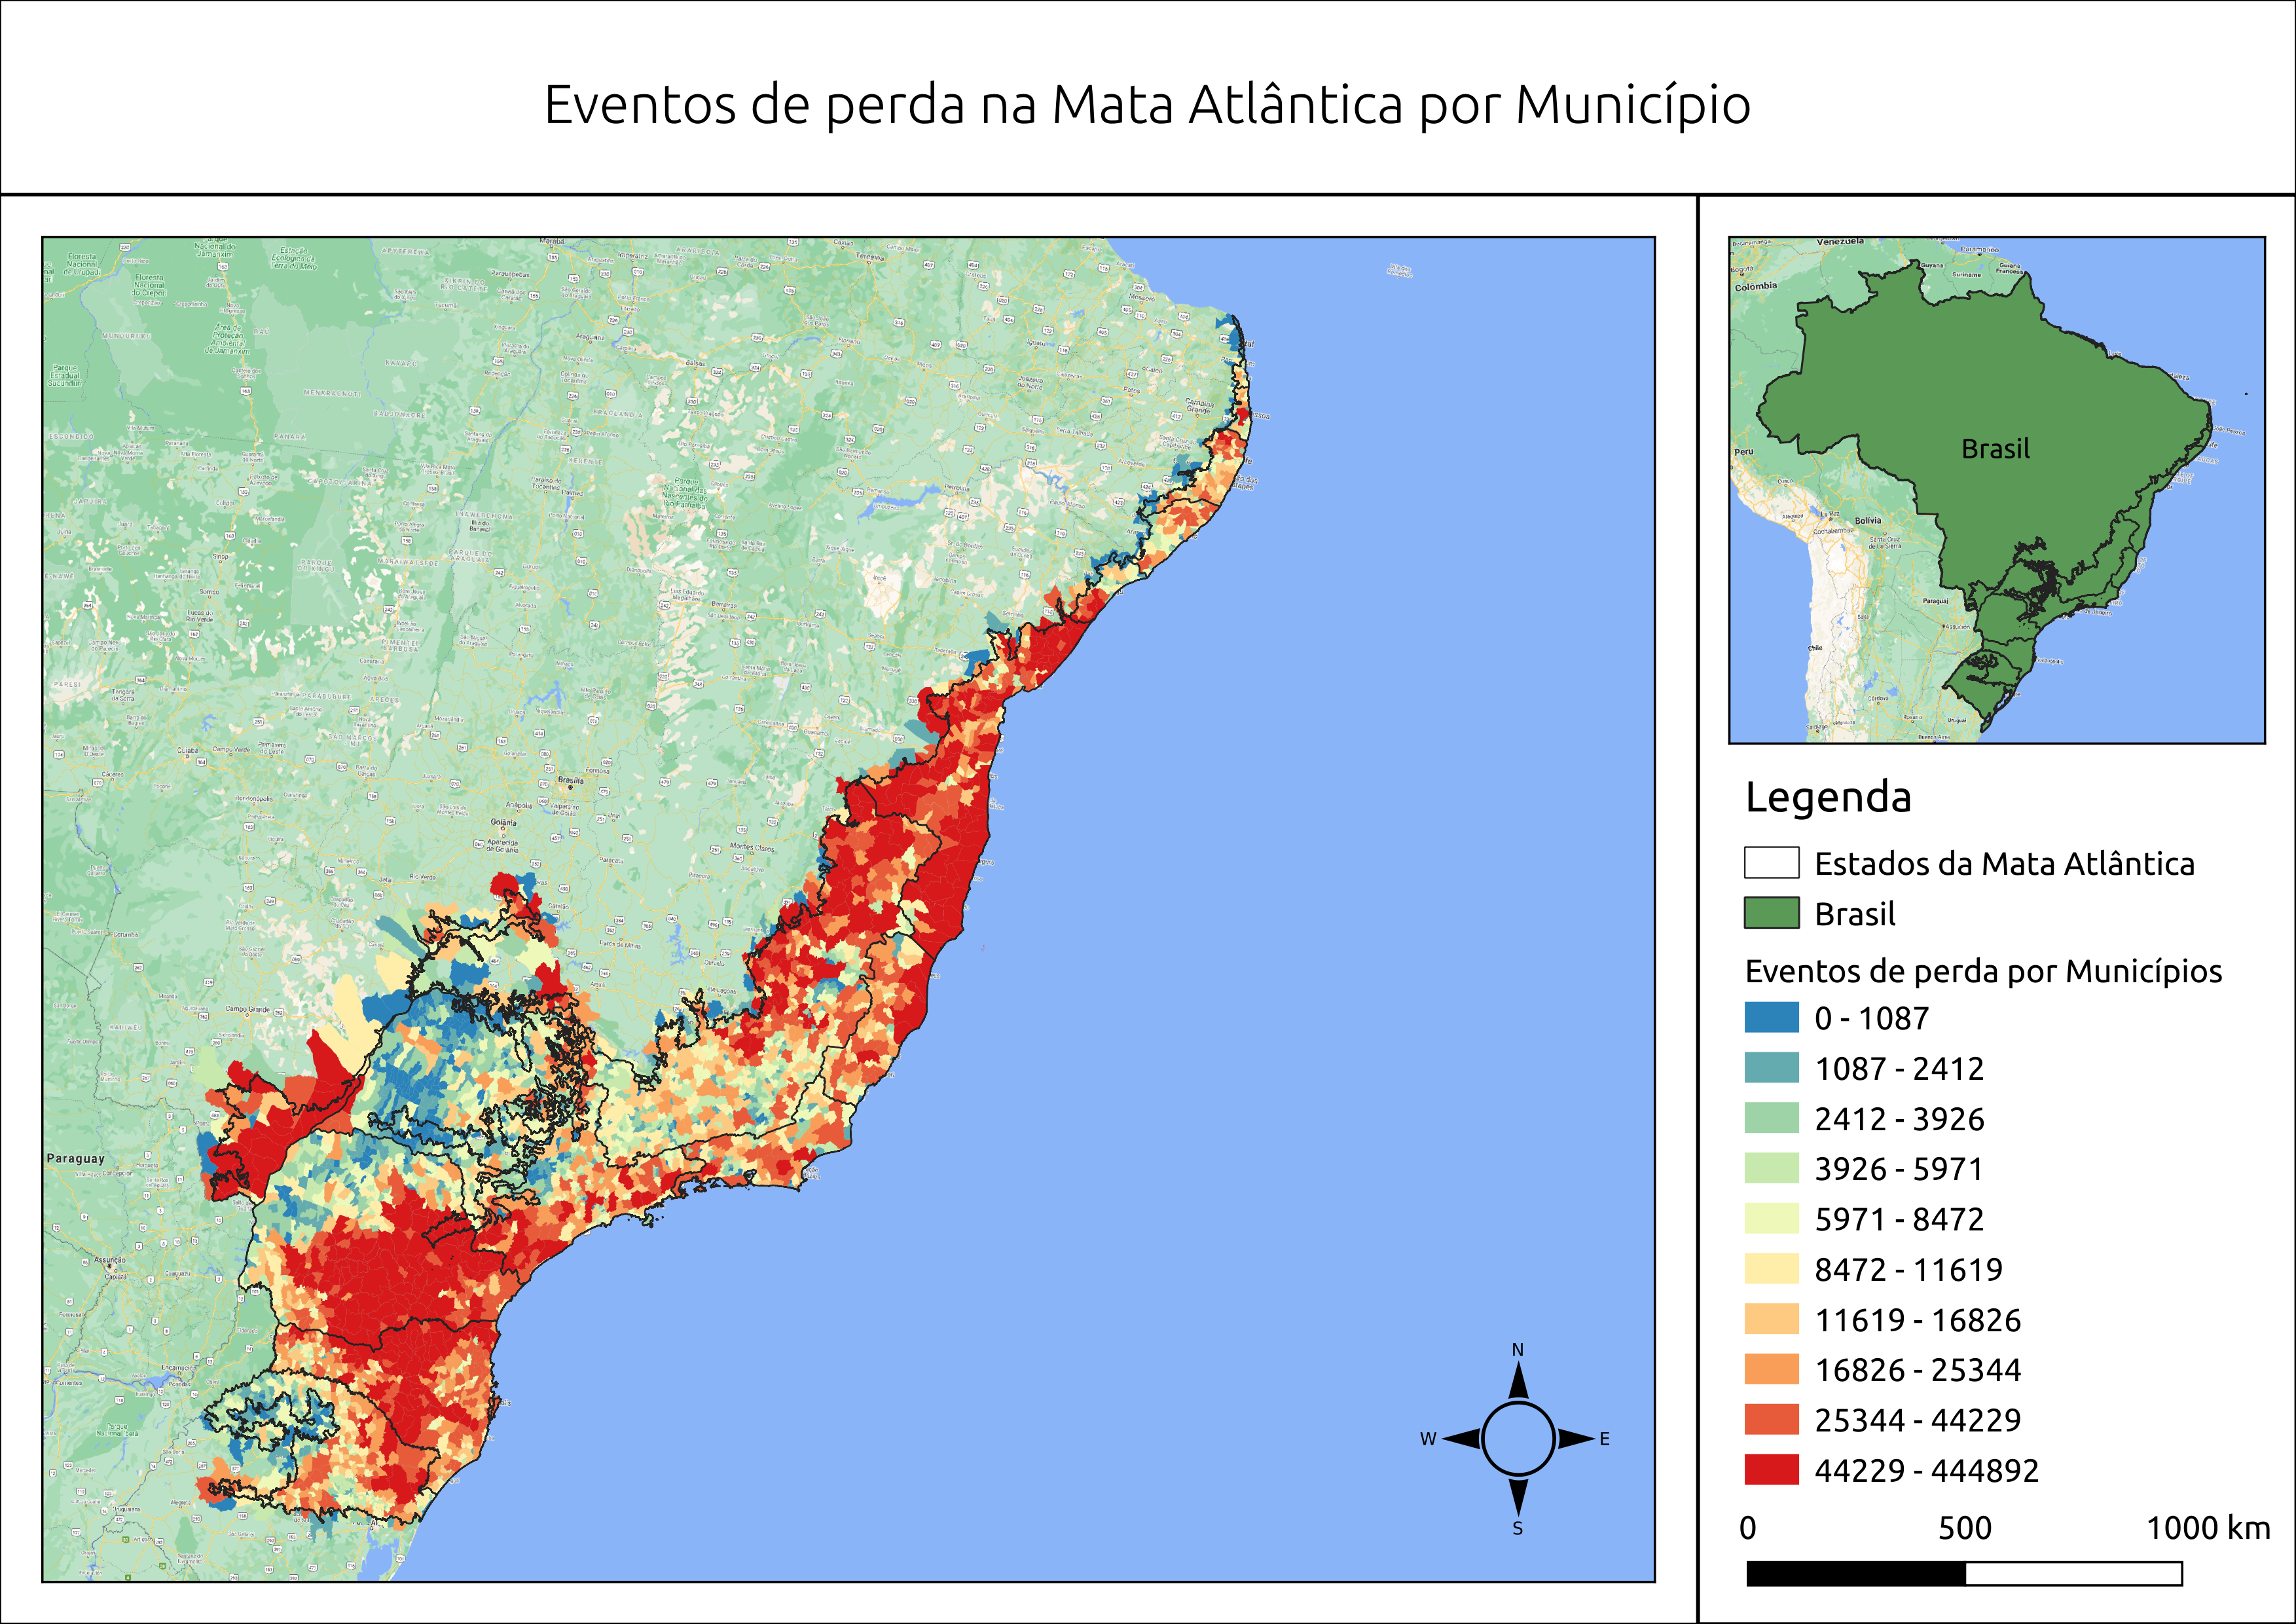
\includegraphics[scale=.5]{images/mun_loss_mun_masked85_maskedgain.png}
    \caption{Todos os eventos de perda na Mata Atlântica entre 1985 e 2018 por município. Os valores representam o número de pixels que tiveram alguma detecção de perda.}
    \label{fig:mun_loss_masked85_maskedgain}
\end{figure}

Seja através dos mapas de calor, ou divisões por municípios ou estados, podemos observar que os eventos de perda na Mata Atlântica brasileira ocorre de forma aglomerada em certas regiões. Apesar de termos registrado eventos de perda em todos os tipos de fitofisionomias, parece ter havido uma predominância de eventos em florestas ombrófilas densas principalmente por conta das perdas detectadas no Paraná, Santa Catarina e Bahia.

\subsubsection{Os eventos de ganho na Mata Atlântica}

\hspace{13pt} Somando-se todos os eventos de ganho detectados pelo algoritmo e após as filtragens necessárias, houveram ao longo de todos os anos da análise 68.869.908 de pixels com um ganho médio de 197 ou aumento de 0.197 no índice NDVI. Isso equivale a uma área total de aproximadamente 62 mil $ km^2 $ de florestas que sofreram ganhos significativos. Como discutido na sessão 3.2.4, áreas de florestas pseudo-invariantes não foram consideradas, sendo assim, esta área representa um ganho real de área verde dentro do bioma. 

Na Figura \ref{fig:heat_gain}, podemos ver que o ganho de áreas no bioma de deu de forma bem mais homogênea que as áreas de perda. Apenas alguns pontos de aglomeração podem ser visualizados como no sul do Rio Grande do Sul, Espírito Santo, sul de Pernambuco, São Paulo e Minas Gerais.

\begin{figure}[H]
    \centering
    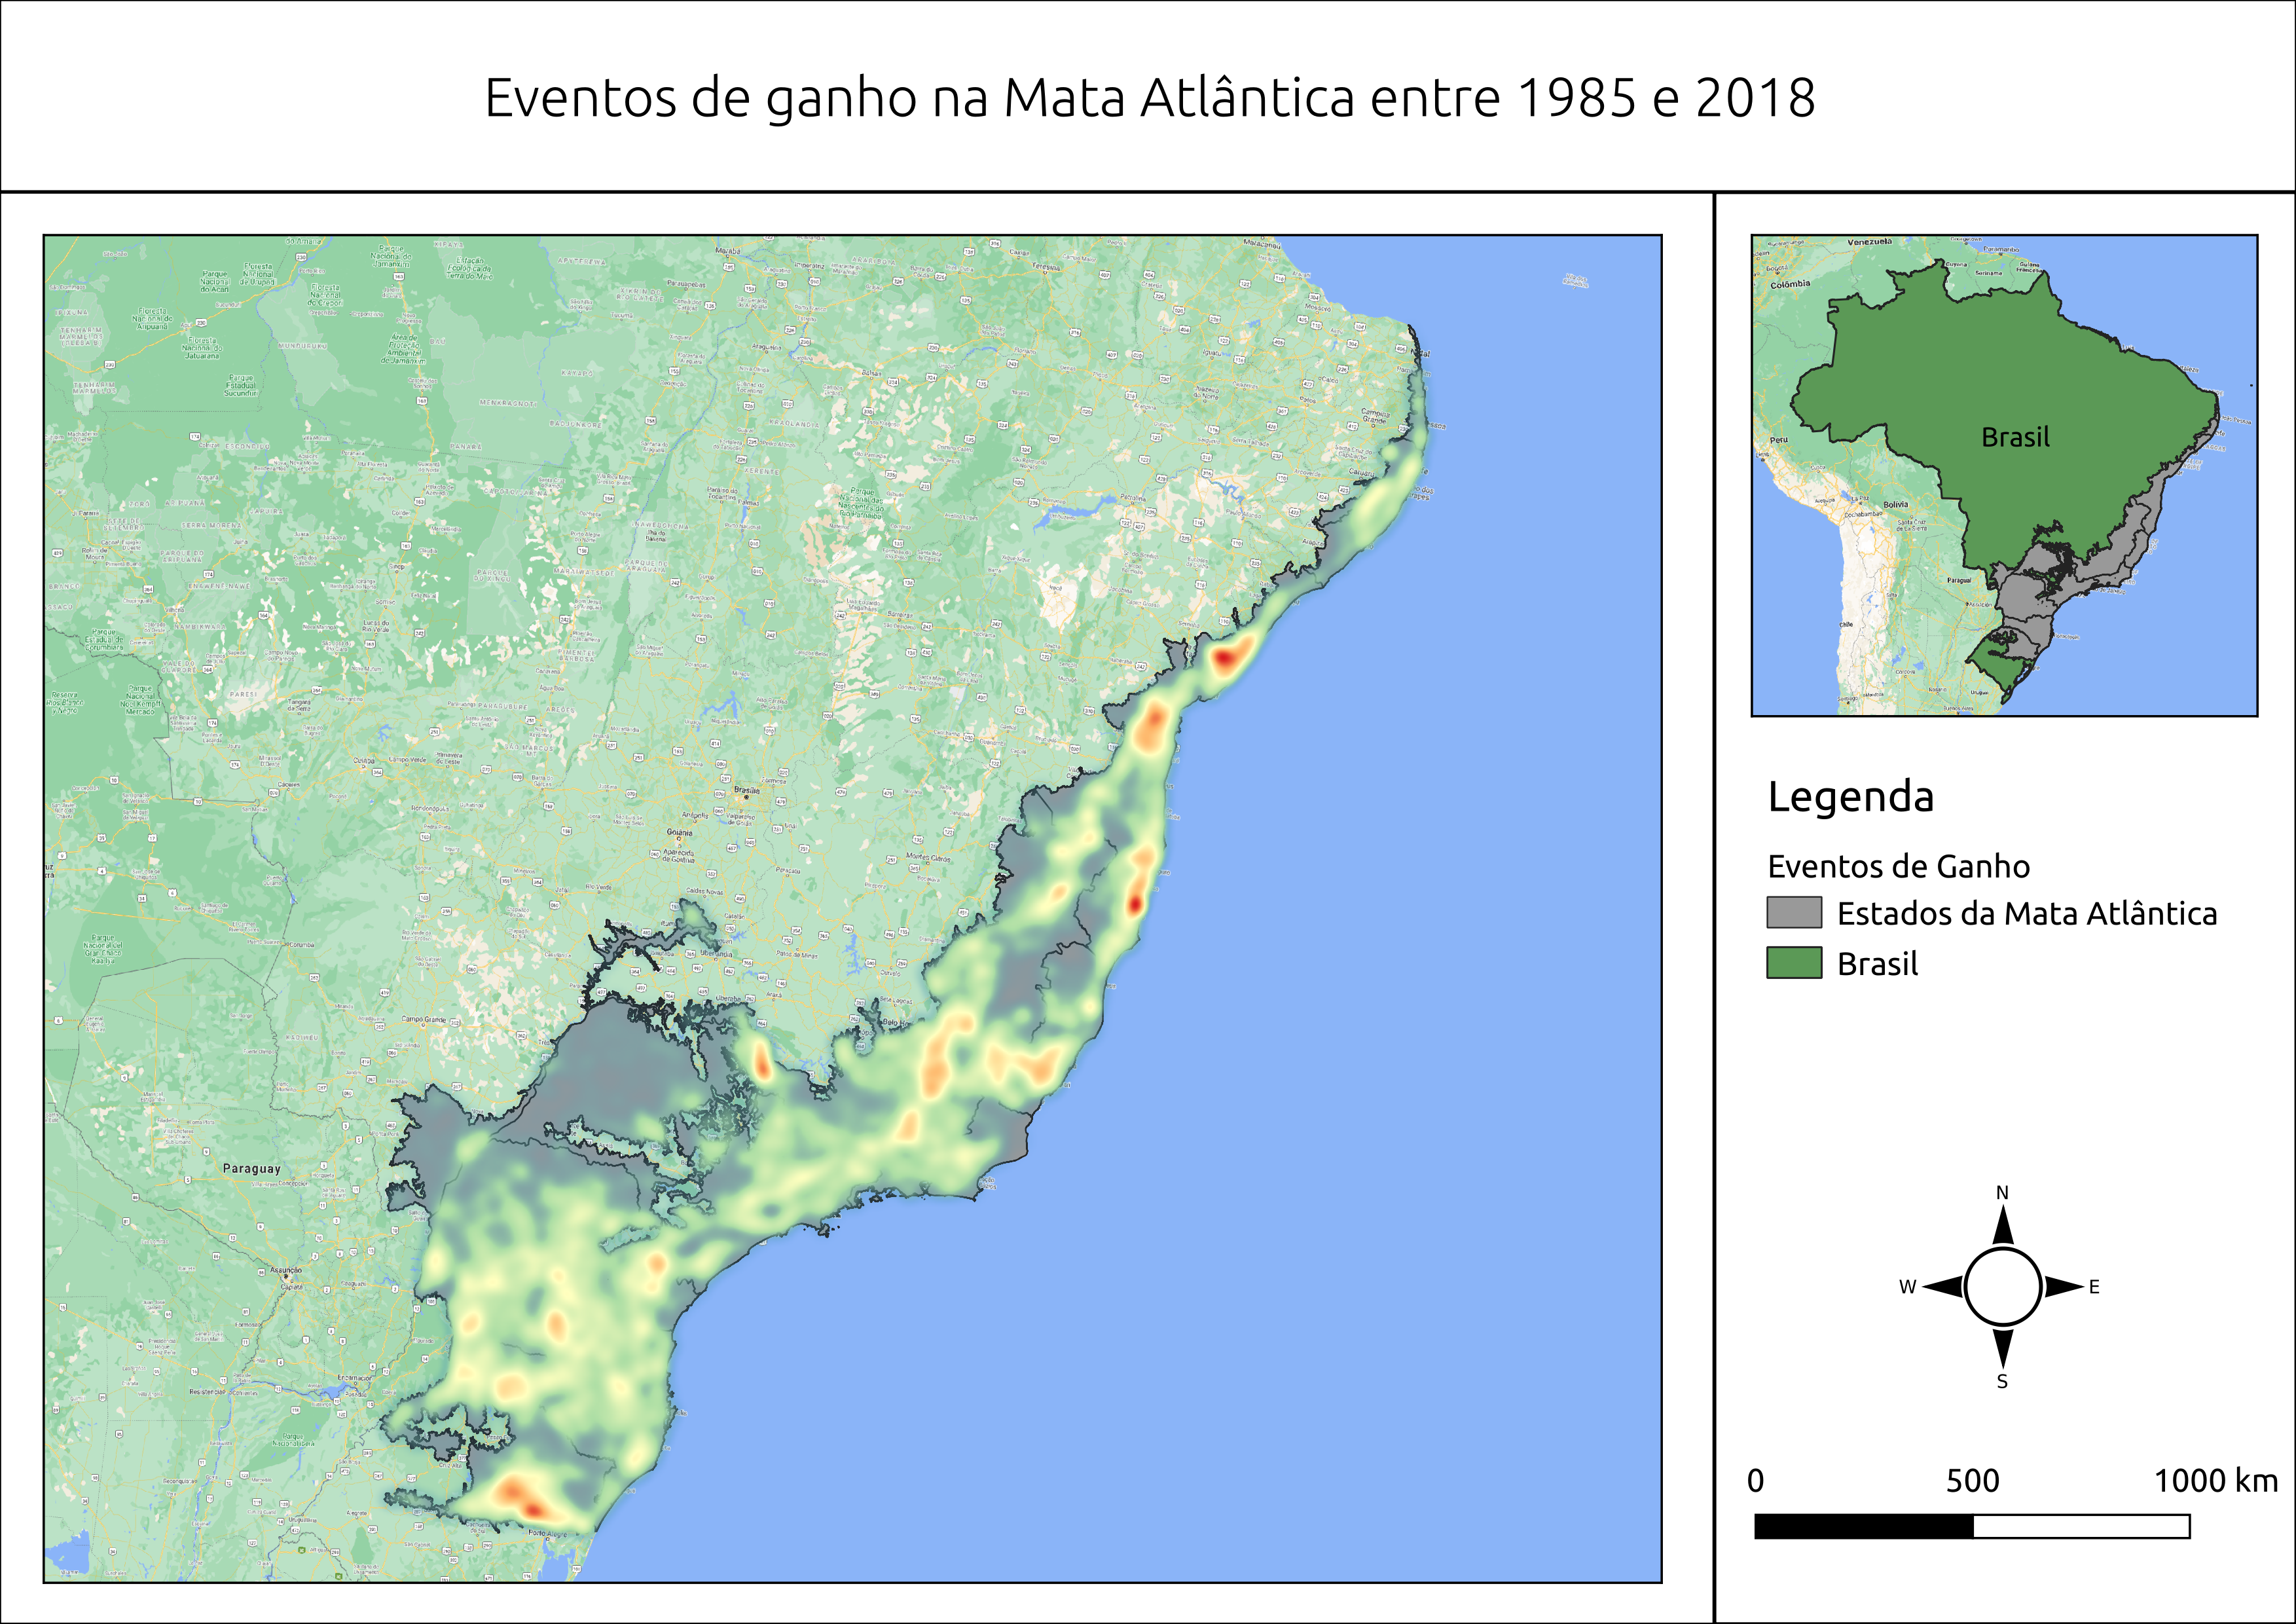
\includegraphics[scale=.5]{images/heatmap_gain_masked18_dur_gt4_inv_for.png}
    \caption{Mapas com os eventos de ganho entre 1985 e 2018.}
    \label{fig:heat_gain}
\end{figure}

Quando analisamos por estado, verificamos que Paraná e Minas Gerais dominam na quantidade total de eventos, seguido de São Paulo, Santa Catarina e Bahia (Figura \ref{fig:estados_gain}). Ao dividir o número de eventos pela área de cada estado vemos que o concentração ocorre principalmente em Santa Catarina e Bahia, seguida de Sergipe, Rio Grande do Sul e Espírito Santo (Figura \ref{fig:estados_gain_proporcional}).

\begin{figure}[H]
    \centering
    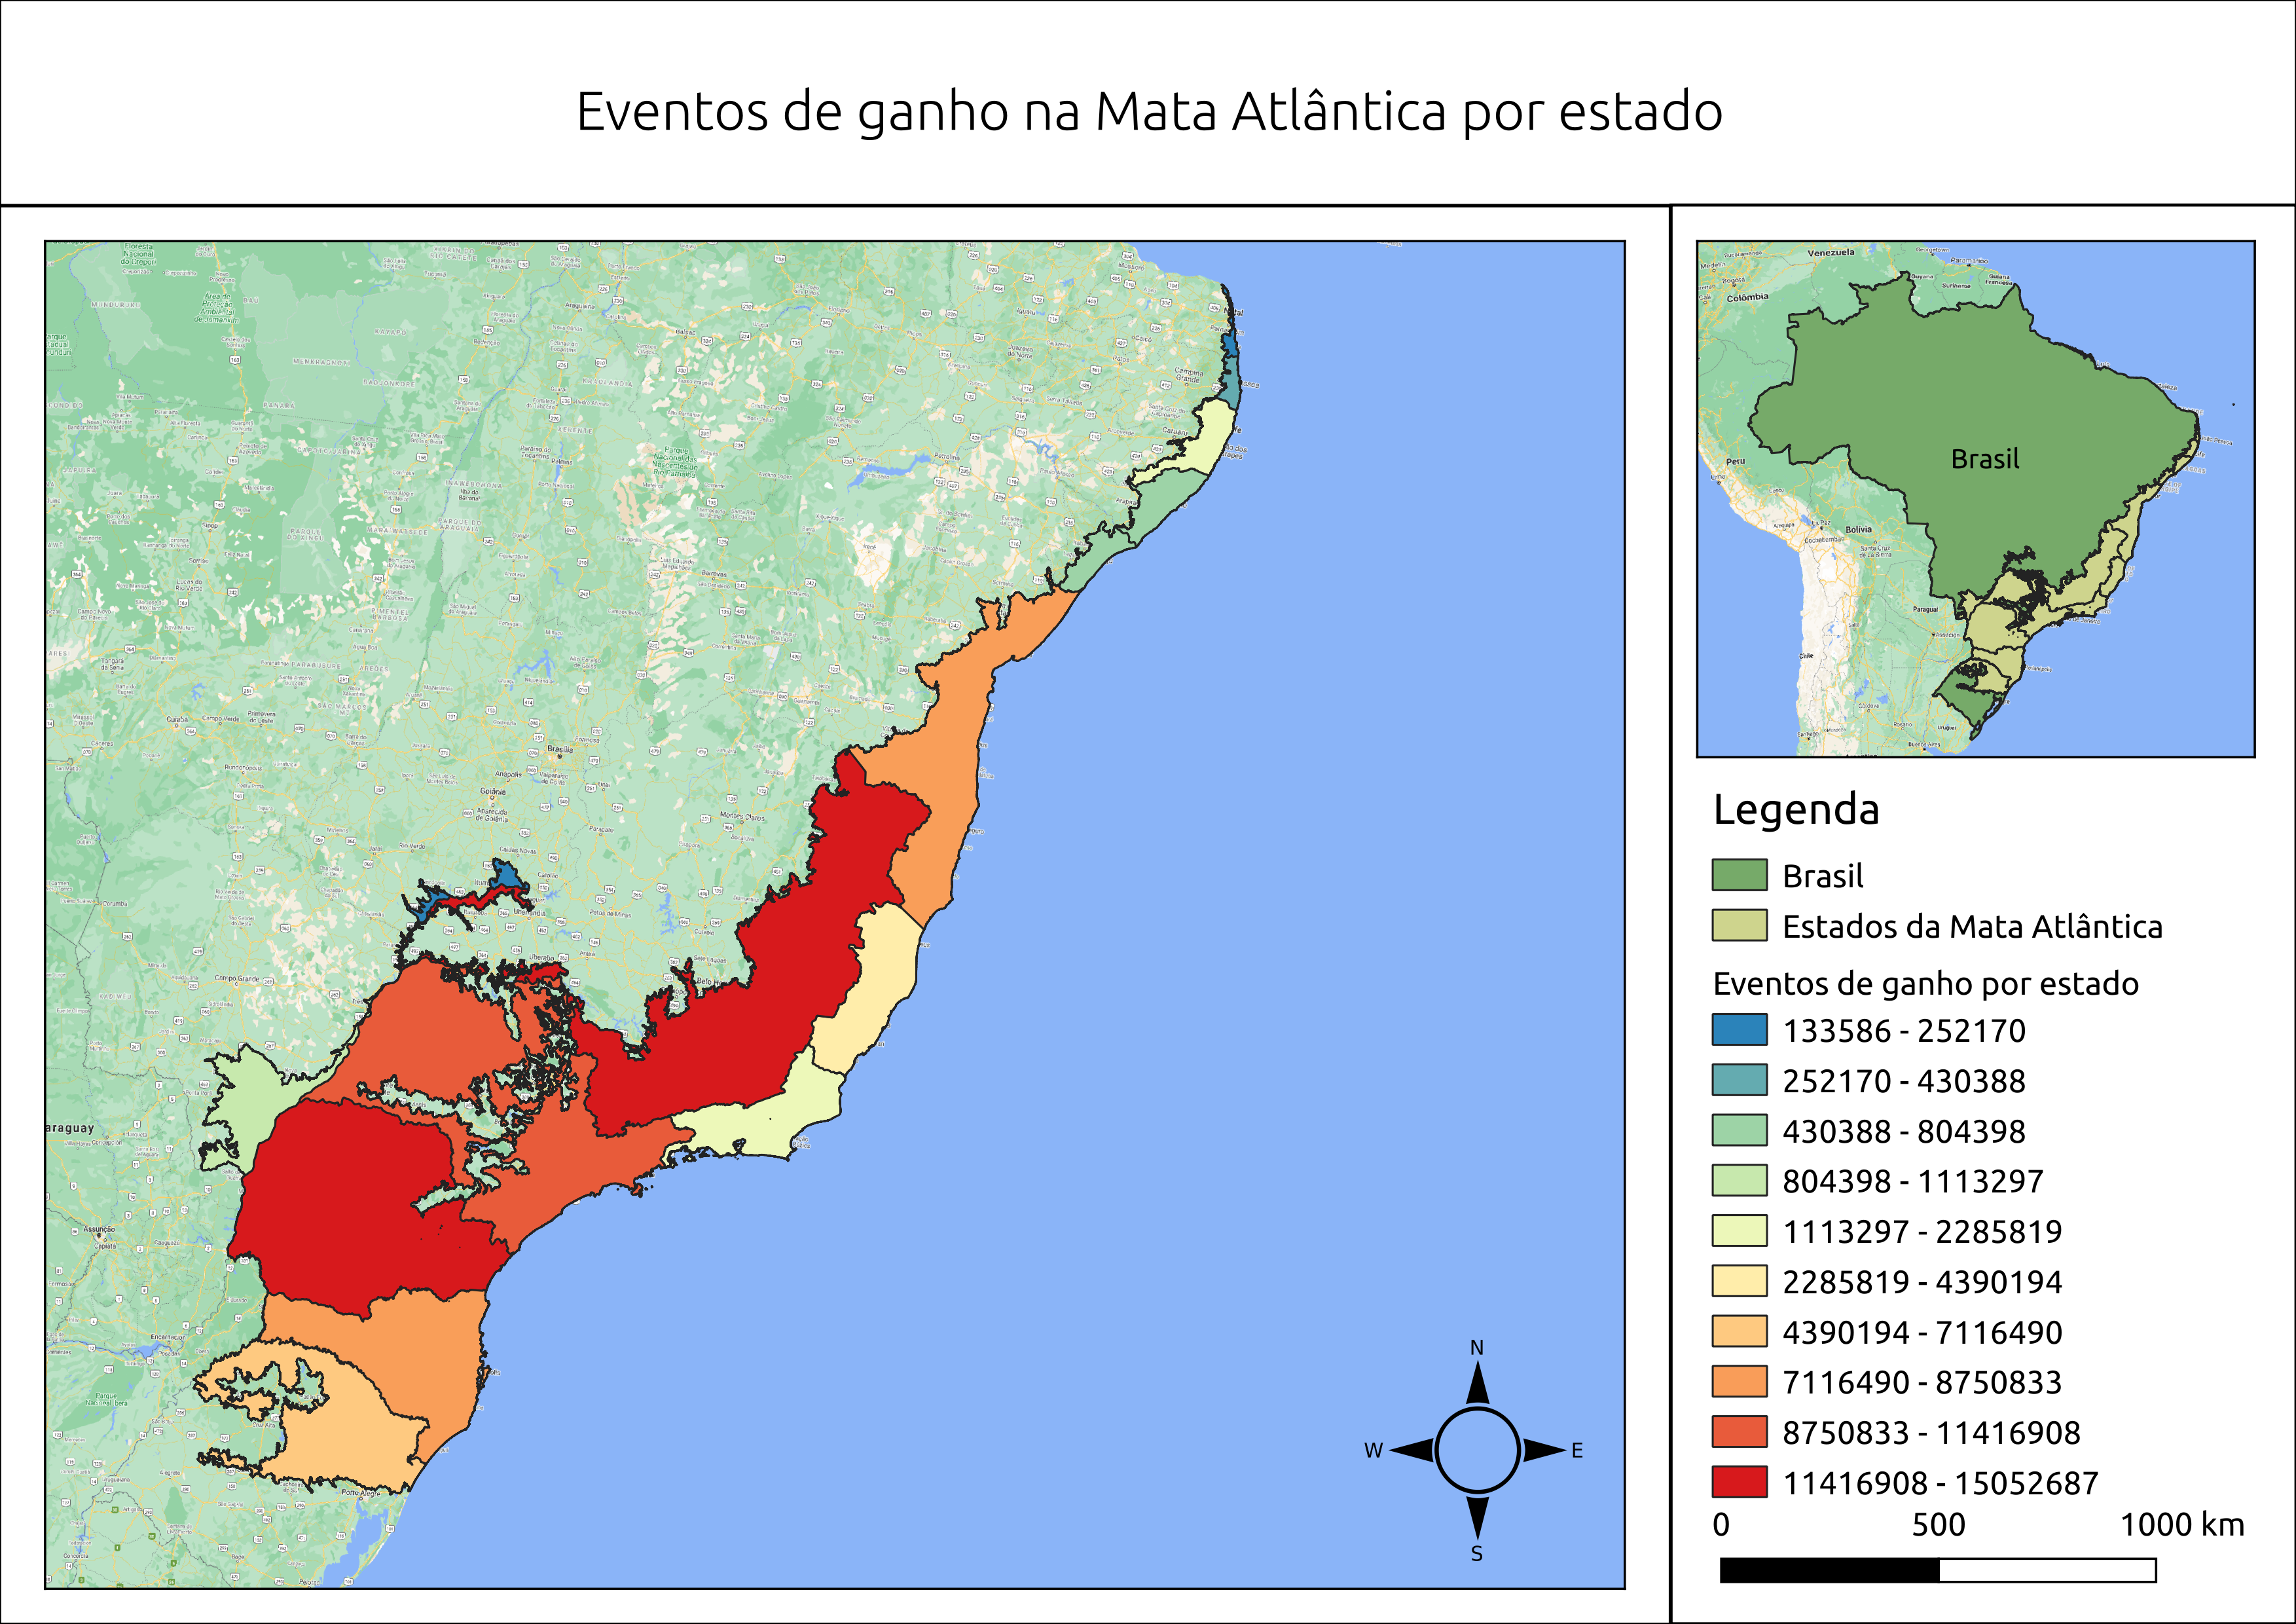
\includegraphics[scale=.5]{images/estados_gain_seg6_masked18_dur_gt4_inv_for.png}
    \caption{Mapas com os eventos de ganho entre 1985 e 2018 por estado. Os valores representam o número de pixels que tiveram alguma detecção de ganho.}
    \label{fig:estados_gain}
\end{figure}

\begin{figure}[H]
    \centering
    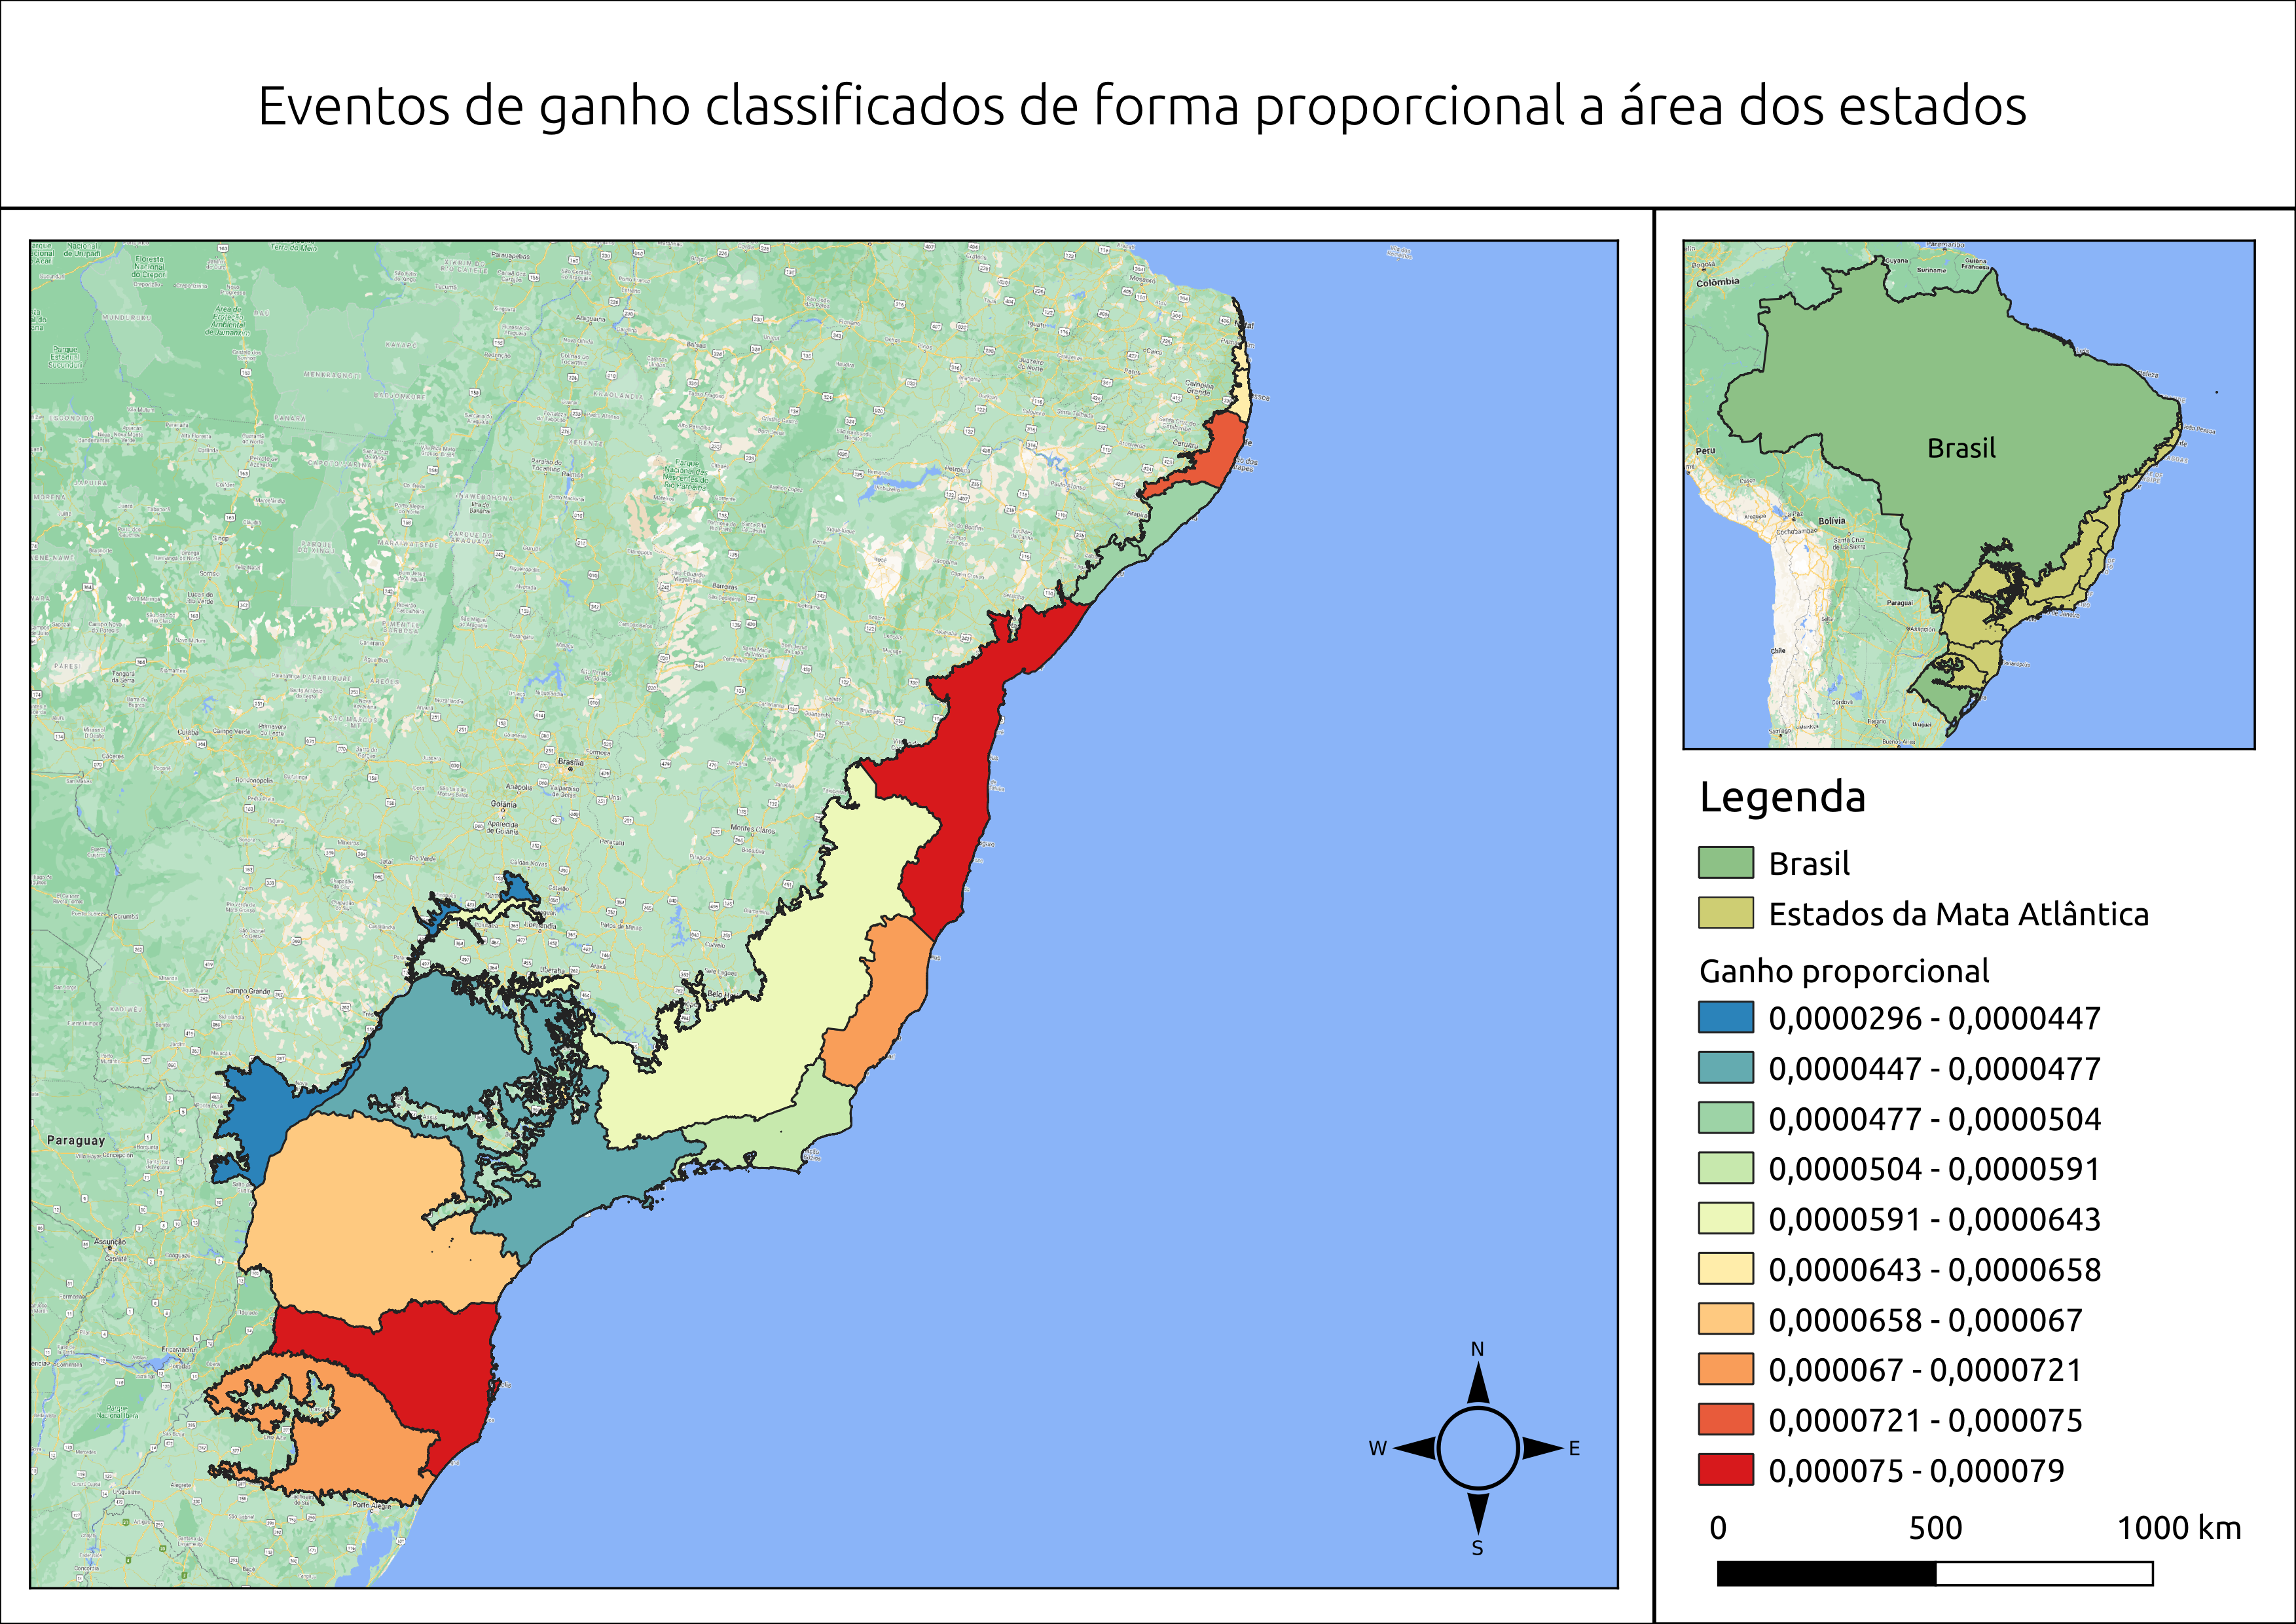
\includegraphics[scale=.5]{images/estado_gain_proporcional.png}
    \caption{Mapas com os eventos de ganho entre 1985 e 2018 classificado de acordo com a proporção de área de cada estado.}
    \label{fig:estados_gain_proporcional}
\end{figure}

Já quando realizamos a análise por município, assim como no cenário de perdas, conseguimos perceber uma maior aglomeração em municípios em estados que tiveram baixa taxa de eventos como o Rio de Janeiro (Figura \ref{fig:mun_gain}). A lista de municípios com a maior quantidade de eventos se mostrou um pouco mais heterogênea que a do cenário de perdas (Tabela \ref{tab:mun_gain}). 

\begin{figure}[H]
    \centering
    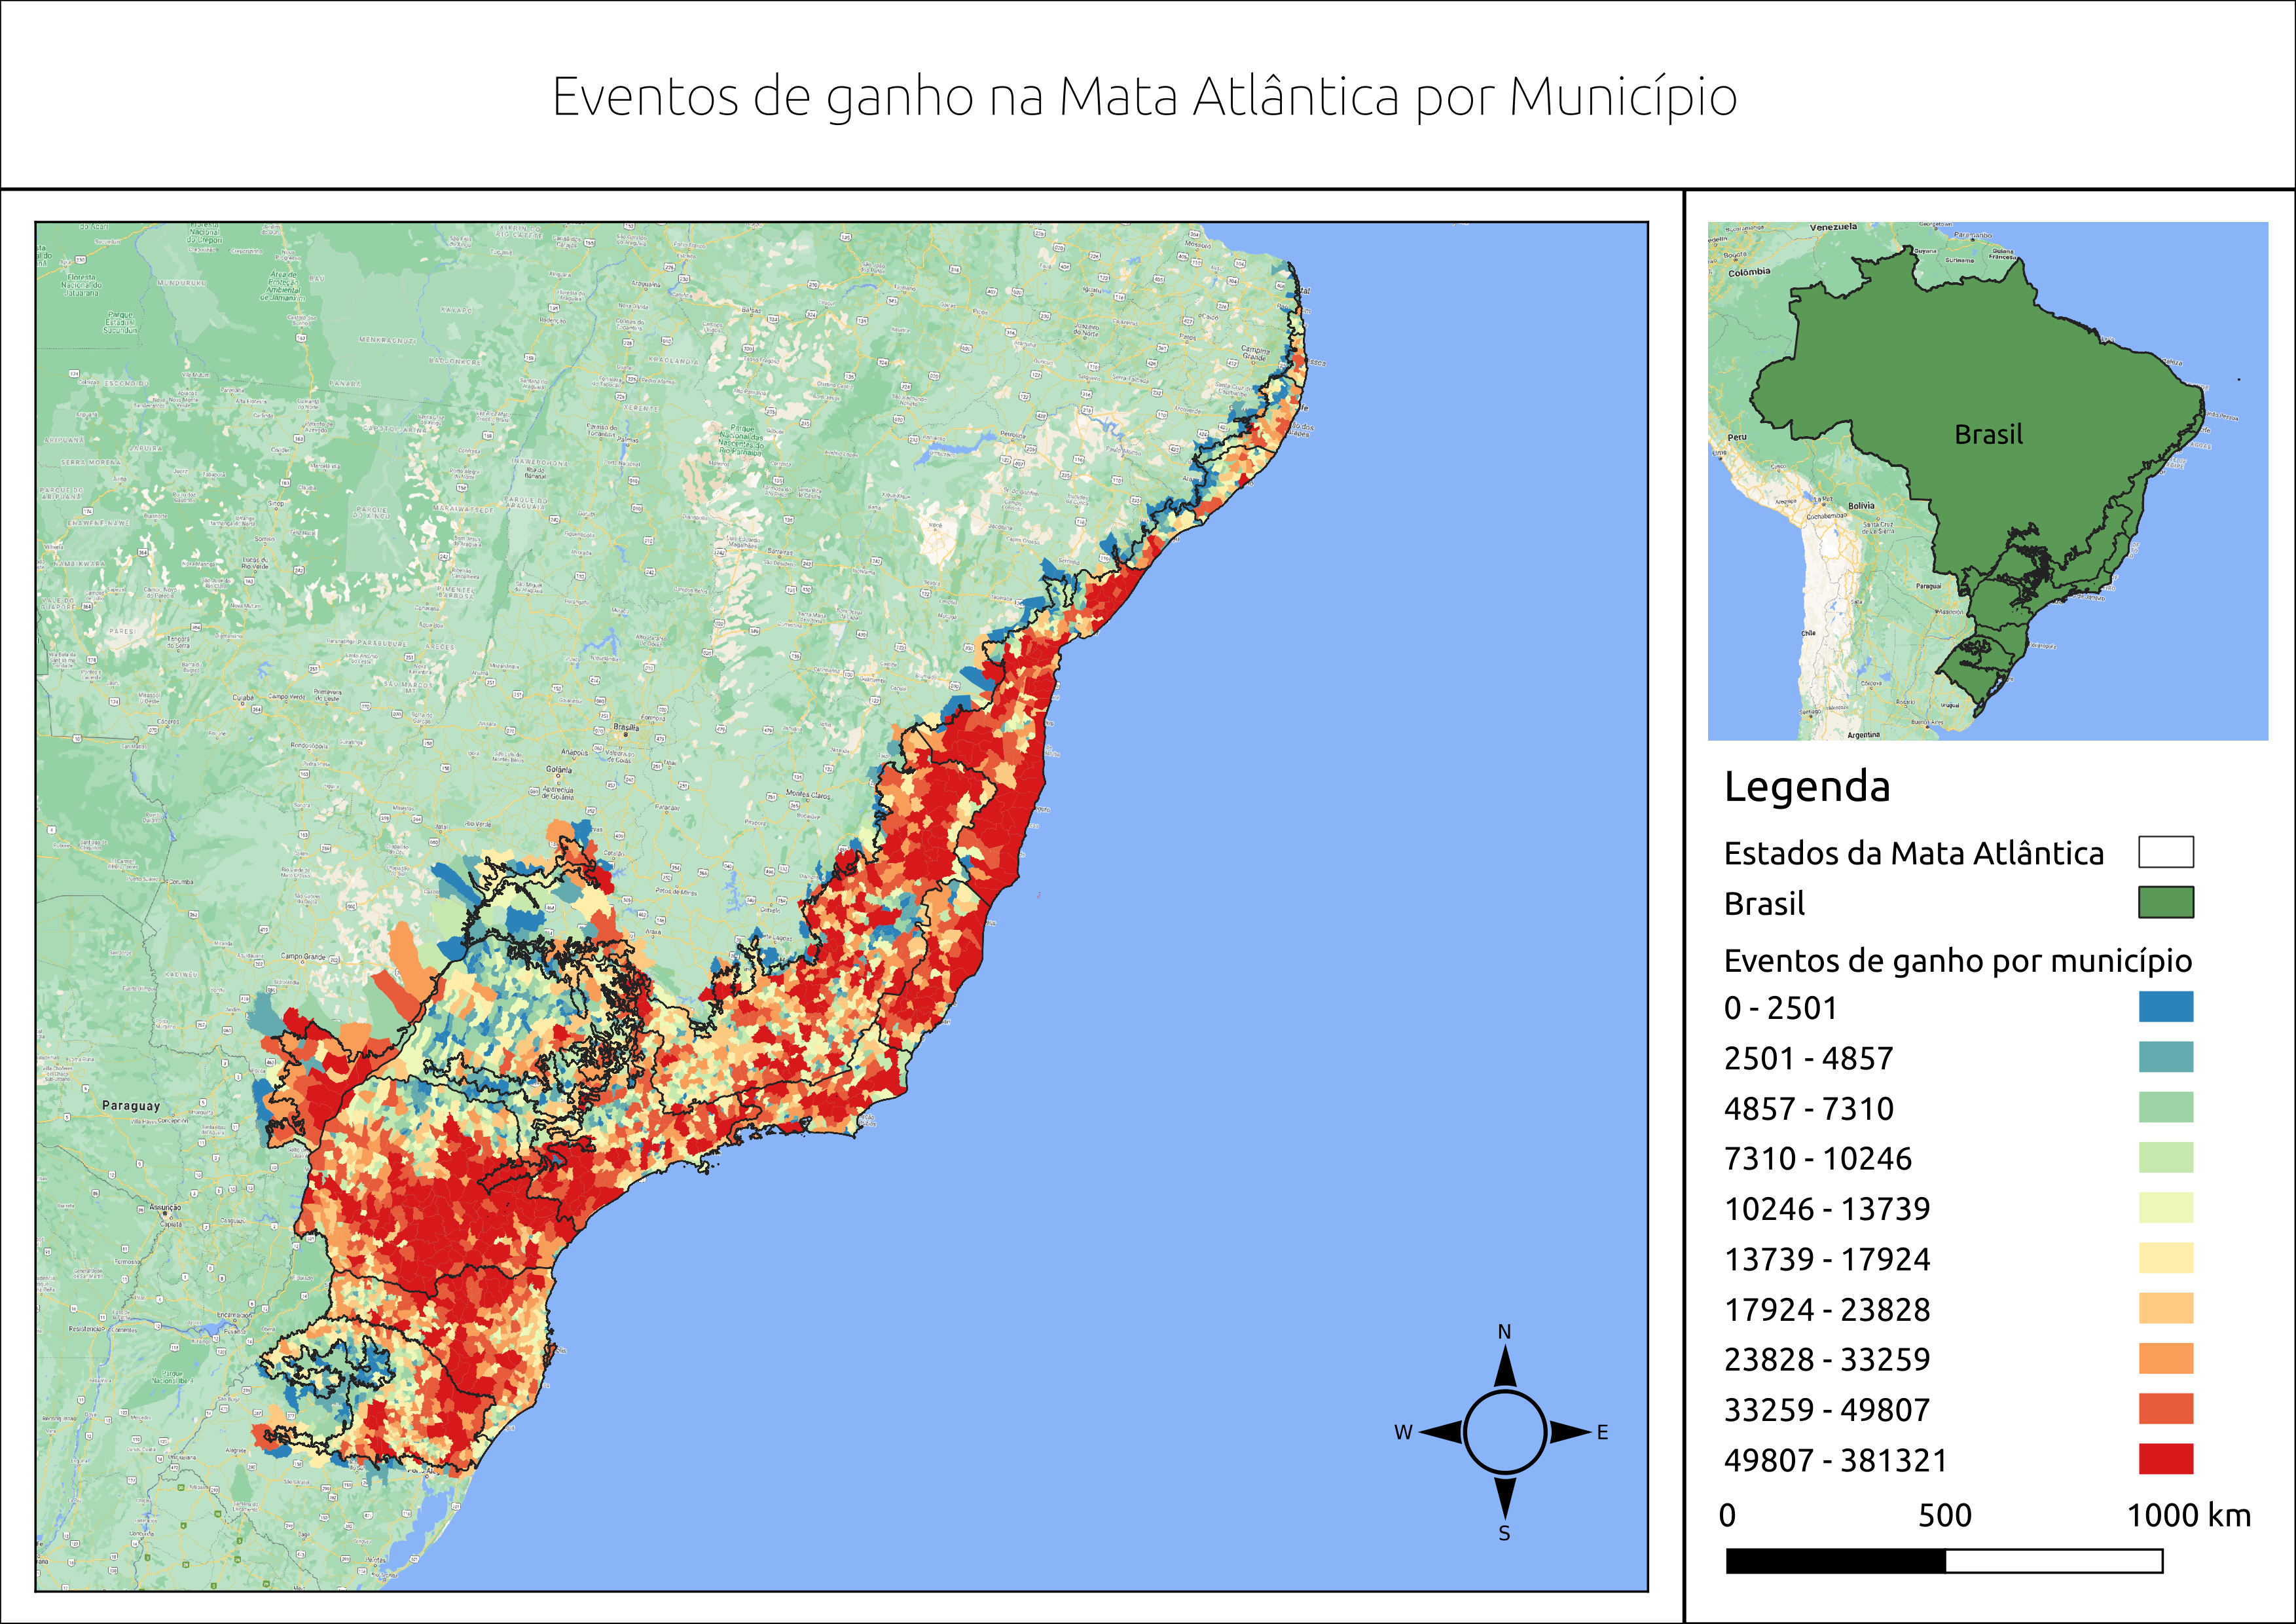
\includegraphics[scale=.5]{images/mun_gain_seg6_masked18_dur_gt4_inv_for.png}
    \caption{Mapas com os eventos de ganho entre 1985 e 2018 por município. Os valores representam o número de pixels que tiveram alguma detecção de ganho.}
    \label{fig:mun_gain}
\end{figure}

\begin{table}[H]
    \centering
    \rowcolors{2}{red!50!yellow!30}{green!40!yellow!10}
    % \footnotesize
    \begin{tabular}{|c | c | c|}
    \hline
                            Nome & Eventos & UF \\
                Porto Seguro & 381321 & BA \\ 
                       Prado & 337864 & BA \\
                Jequitinhonha & 309792 & MG \\
        Santa Cruz Cabrália & 243153 & BA \\
                    Linhares & 241735 & ES \\
                      Almenara & 235791 & MG \\
              Prudentópolis & 231492 & PR \\
                    Belmonte & 228173 & BA \\
                  Guarapuava & 225197 & PR \\
                  Ortigueira & 218987 & PR \\
                  Entre Rios & 203945 & BA \\
                   Cruz Machado & 196431 & PR \\
            Domingos Martins & 182013 & ES \\
                 Juiz de Fora & 181554 & MG \\
                   Esplanada & 181265 & BA \\
                      Mariana & 177423 & MG \\
               Teófilo Otoni & 176573 & MG \\
                      Tibagi & 175646 & PR \\
  São Sebastião do Paraíso & 175471 & MG \\
                   Caravelas & 174156 & BA \\
    \hline
    \end{tabular}
    \caption{Os vinte municípios com maior número de eventos de perda}
    \label{tab:mun_gain}
\end{table}




\subsection{Discussões finais e conclusão}

\hspace{13pt} Percebemos que o algoritmo apresentou uma boa resposta quando aplicado a contextos de floresta tropical. Mesmo utilizando o Landtrendr com um mesmo conjunto de parâmetros em fitofisionomias que apresentam respostas espectrais com comportamento médio estatisticamente diferentes, o resultado aparentou ser bastante satisfatório. Ainda será necessário realizar um processo de validação nos resultados obtidos para entender melhor o grau e confiança desses resultados.

Apesar da facilidade de uso do Landtrendr em plataformas como o GEE, não se pode dizer que a aplicação do algoritmo é trivial, já que o mesmo possui um custo de processamento elevado mesmo na plataforma do Google. Esta característica acaba gerando a necessidade de códigos um pouco mais complexos, uma capacidade de armazenamento maior e um tempo total de processamento relativamente alto. No entanto, quando comparado a técnicas mais tradicionais, a utilização da técnica ainda apresenta benefícios significativos. Todo o trabalho de pré-processamento e criação de composições processadas como dado de entrada é feito com apenas uma única função, e a escolha dos parâmetros pode ser feita de forma rápida tanto dentro da plataforma como em aplicativos web criados especialmente para a realização de testes. 

Os testes prévios são essenciais, já que o bom resultado do algoritmo está diretamente ligado aos parâmetros utilizados e principalmente a banda/índice que é processada para identificar as mudanças. Estudos mais recentes buscaram entender o comportamento do algoritmo em relação as bandas utilizadas e também houve o desenvolvimento e adição de uma nova camada gerada pelo algoritmo além das camadas de resultado já tradicionais chamada DSNR (\textit{Disturbance Signal-to-Noise Ratio}) \citep{COHEN2018131}. Com camadas como a DSNR, as difenreças encontradas na aplicação do algoritmo em áreas temperadas e tropicais fica ainda mais clara. 

Já para o processo de validação será necessário a utilização da ferramenta TimeSync \citep{COHEN20102911}, desenvolvida pelo mesmo grupo de pesquisadores do Landtrendr. A validação utilizando o TimeSync infelizmente ainda é pouco otimizada e necessita de muitas dependências externas para seu funcionamento. No entanto, ainda é a melhor ferramenta de validação de séries temporais. Algumas áreas em diferentes fitofisionomias serão utilizadas para a coleta de amostras e posteriormente processadas na plataforma.

Muitas perguntas já puderam ser respondidas através dessa análise, mas outras ainda precisam ser entendidas. Além da validação que servirá de base para a compreensão real da viabilidade da aplicação do algoritmo em ambientes tropicais extensos, ainda será necessário realizar outras análises como o comportamento das unidades de conservação do bioma, assim como o cálculo da idade das florestas secundárias no bioma. 